\section{Einführung}
\label{Einführung}
\subsection{Relevanz \& Problemstellung}
Bessere Code-Qualität mit vergleichbar minimal erhöhtem Zeitaufwand ist ein erstrebenswertes Ergebnis und das Ziel von Test-driven Development (TDD). Durch die Idee von TDD -- nämlich kurze Iterationen von:
\begin{enumerate}
  \item Tests schreiben
  \item Tests ausführen und fehlschlagen lassen
  \item Code implementieren
  \item Tests ausführen und den Code eventuell weiter implementieren, bis die 
  Tests nicht mehr fehlschlagen
  \item Tests und Code refactoren
  \item Tests erneut ausführen
\end{enumerate}
wird eine hohe Testabdeckung und ein sauberer Code durch das Refactoring erzielt.

AngularJS ist ein umfassendes Model-View-Whatever (MVW) Framework und bringt viele eigene Komponenten mit sich, wie beispielsweise Directives und Services. Um test-driven mit AngularJS entwickeln zu können, ist es wegen der Vielfalt der eigenen Komponenten relevant, alle diese Komponenten testen zu können.

Aus der Relevanz von TDD mit AngularJS ergibt sich die Problemstellung der Auswahl eines passenden Testing Frameworks. Jasmine und Mocha sind zwei JavaScript Testing Frameworks, welche sich für diese Aufgabenstellung anbieten. Deshalb werden beide Frameworks in dieser Arbeit gegenüber gestellt und analysiert, um die Unterschiede beziehungsweise die Vor- und Nachteile der beiden Frameworks darstellen zu können.

\subsection{Methodenüberblick}
\begin{itemize}
  \item \textbf{Test-driven Development (TDD)}: Eine theoretische Einführung in TDD ist grundlegend für den weiteren Inhalt der Arbeit.
  \item \textbf{AngularJS}: AngularJS wird zusammen mit den dazugehörigen Komponenten theoretisch und praktisch dargestellt Theorie und Praxis arbeiten hier sehr dicht zusammen, um im Vorfeld alle Facetten des MVC/W-Frameworks abzuklären.
  \item \textbf{Testing Frameworks}: Um abklären zu können, welches der beiden JavaScript Testing-Frameworks {\glqq Jasmine\grqq} und {\glqq Mocha\grqq} besser geeignet ist, um alle Eigenschaften von AngularJS abzudecken, wird ein direkter theoretischer Vergleich der Frameworks und deren Eigenschaften gegeben. Darüber hinaus wird eine Applikation test-driven mit beiden Frameworks entwickelt. Die Applikation wird alle der relevanten Eigenschaften von AngularJS behandeln.
\end{itemize}

\subsection{Forschungsfrage}
Wie ist der aktuelle Stand der test-driven Entwicklung mit AngularJS und welches der beiden JavaScript Testing-Frameworks {\glqq Jasmine\grqq} und {\glqq Mocha\grqq} ist besser geeignet für diesen Zweck?

\subsection{Praxis}
Alle Praxisbeispiele befinden sich im GitHub-Repository \glqq{https://github.com/Calvitium/tdd-angularjs-jasmine-vs-mocha\grqq} im Verzeichnis \glqq{source\grqq} und können jederzeit eingesehen werden.

Folgende Unterverzeichnisse sind relevant:
\begin{itemize}
  \item \glqq{\textbf{simple-tests}\grqq}: Hier sind die Praxisbeispiele zu TDD in JavaScript zu finden. Um diese ausführen zu können, müssen die npm\footnote{https://www.npmjs.org/}-Pakete \glqq{karma\grqq}, \glqq{karma-jasmine\grqq} und \glqq{karma-phantomjs-launcher\grqq} global installiert werden.
  \item \glqq{\textbf{marvel-super-heroes-tdd-jasmine}\grqq} beziehungsweise \glqq{\textbf{marvel-super-heroes-tdd-mocha}\grqq}: Hier befindeen sich die mit Jasmine und Mocha test-driven entwickelten AngularJS Applikationen. Um die Applikationen und Tests ausführen zu können, müssen das npm-Paket \glqq{grunt-cli\grqq}\footnote{http://gruntjs.com/} und eine MongoDB\footnote{http://www.mongodb.org/} Datenbank global installiert sein, und in jedem Verzeichnis \glqq{npm install\grqq} sowie \glqq{bower install\grqq} ausgeführt werden. Danach kann im jeweiligen Verzeichnis via Grunt die Applikation gestartet (grunt serve) oder die Tests ausgeführt (grunt test) werden.
\end{itemize}

\newpage

\section{Testen in der Webentwicklung}
\subsection{Manuelles und automatisiertes Testen}
In der Webentwicklung gibt es laut \cite[3]{Johansen:2011} ein Test-Schema, welches jeder/m EntwicklerIn bekannt sein dürfte:
\begin{enumerate}
  \item Code schreiben
  \item in den Browser wechseln und aktualisieren
  \item die geschriebenen Änderungen überprüfen
  \item wiederholen
\end{enumerate}
Wird dieses Schema angewandt, so spricht man von \glqq{manuellem\grqq} Testen. Manuelles Testen ist jedoch zeit-intensiv, nicht reproduzierbar und fehleranfällig \autocite[3]{Johansen:2011}. Wenn eine Webapplikation manuell getestset wird, und es kommt zu einer Änderung, so muss jegliche Funktionalität, welche von der Änderung abhängt oder beinflusst wird, ebenfalls manuell getestet werden. Dazu kommt noch, dass unterschiedliche Browser JavaScript unterschiedlich interpretieren, dass heißt, es müssen alle Änderungen manuell in mehreren Browsern getestet werden. Eine erhöhte Fehleranfälligkeit erklärt sich dadurch, dass es nicht ausschließbar ist, dass bei dem einen oder anderen manuellen Test, etwaige Eventualitäten übersehen werden, welche bei vorhergehenden Durchläufen getestet wurden.

Dem manuellen Testen steht das automatisierte Testen gegenüber. Beim automatisierten Testen werden Tests geschrieben, welche die Korrektheit einer Software, beziehungsweise einer Software-Komponente, überprüfen sollen. Wenn eine Änderung stattfindet, werden die geschriebenen Tests ausgeführt und die/der EntwicklerIn erhält direkt positives oder negatives Feedback. Automatisiertes Testen ermöglicht es, Tests zu reproduzieren, und ist somit auch nicht so zeit-intensiv wie manuelles Testen. Die Tests sorgen darüber hinaus für eine geringere Fehleranfälligkeit, da immer alle Tests ausgeführt werden und somit auch keine Eventualität, welche beim letzten Durchlauf getestet wurde, übersehen wird.

Da das Test-Schema des manuellen Testens auf Dauer zu viele Probleme mit sich bringt, wurden laut \cite[xix]{Johansen:2011} viele Tools, welche aus anderen Programmiersprachen bekannt sind, entwickelt, um JavaScript-EntwicklerInnen das Programmieren zu vereinfachen. Dieses Tools sind beispielsweise Debugger, Profiler oder Testing-Frameworks. Testing-Frameworks, wie beispielsweise \glqq{Jasmine\grqq} oder \glqq{Mocha\grqq}, bieten die notwendige Funktionalität an, um JavaScript automatisiert Testen zu können.

Auch das Ausführen der Tests wird vereinfacht. Um den Entwicklungsprozess optimieren zu können, ist es bei einigen JavaScript-IDEs (Integrated Development Environment, beispielsweise \glqq{WebStorm\grqq}\footnote{http://www.jetbrains.com/webstorm/}) möglich, die Tests via Shortcut zu starten. Wenn keine IDE, sondern ein simpler Code-Editor (wie \glqq{Sublime-Text\grqq}\footnote{http://www.sublimetext.com/}) bevorzugt wird, bieten einige Frameworks die Möglichkeit an, gewisse Code- und Test-Dateien auf Änderungen zu überwachen. Wenn eine Änderung durchgeführt wurde, werden automatisch alle Tests durchgeführt.

Ein weiteres Tool, um das automatisierte Testen von JavaScript zu vereinfachen, ist ein \glqq{Test-Runner\grqq} -- beispielsweise \glqq{Karma\grqq}\footnote{http://karma-runner.github.io/0.12/}. Ein Test-Runner startet einen oder mehrere Browser und führt die geschriebenen Tests in diesem/n aus. Dadurch wird auch die Problematik der unterschiedlichen JavaScript-Interpretation gelöst, denn es können gleichzeitig verschiedene Browser gestartet werden.

Um die Testzeit minimieren zu können, gibt es die Möglichkeit, einen \glqq{headless\grqq} Browser (zum Beispiel \glqq{PhantomJS\grqq}\footnote{http://phantomjs.org/}) zu verwenden. Ein headless Browser verfügt im Gegensatz zu einem normalen Browser über keine Präsentation des \glqq{Document Object Models\grqq} (DOM) und ist somit schneller.

Es wurden also viele Tools geschaffen, um automatisiertes Testen in der Webentwicklung ermöglichen zu können. \cite[xix]{Johansen:2011} schreibt deshalb unter anderem: \textit{\glqq{..., JavaScript has grown up.\grqq}}

\subsection{Arten von Tests}
\subsubsection{Unit-Tests}
Ein Unit-Test ist Code, der produktiven Code testet. Er besteht aus bestimmten Objekten in bekannten Stati. Die Objekte, wie beispielsweise Funktionen, werden ausgeführt. Danach werden sie inspiziert und/oder auf die Richtigkeit überprüft. Der produktive Code wird in Isolation getestet.

Im Vergleich zu Integration-Tests ist es für Unit-Tests wichtig, dass sie isoliert ausgeführt werden -- kein Test soll von einem anderen Test abhängig sein \autocite[4]{Johansen:2011}. Langsame Unit-Tests wirken sich negativ auf das Testen sowie den TDD-Prozess aus. EntwicklerInnen werden langsame Tests nicht so oft ausführen wie schnelle Tests. Insbesondere im Zusammenhang mit TDD bedeuten langsame Tests einen längeren Abstand zwischen den TDD-Zyklen (siehe Kapitel \glqq{3.3 Der TDD-Kreislauf\grqq}). EntwicklerInnen müssen lange auf Feedback warten und werden aus dem Zyklus gerissen.

Unit-Tests können zu jeder Zeit ausgeführt werden, ...
\begin{itemize}
  \item ... um bei einer fertigen Implementierung deren Korrektheit bestätigen.
  \item ... um bei Änderungen Fehler auszuschließen.
  \item ... um bei dem Hinzufügen von neuen Komponenten zu garantieren, dass das System noch vollständig und richtig funktioniert.
\end{itemize}

\subsubsection{Integration-Tests}
Um beispielsweise eine Uhr zu testen, benötigt man beides, Unit- sowie Integration-Tests. Unit-Tests sind für das Testen der einzelnen Zahnräder der Uhr zuständig. Diese werden isoliert auf ihre Korrektheit getestet. Integration-Tests hingegen testen, wie die Zähne der einzelnen Zahnräder ineinandergreifen und ob die Uhr als ganzes richtig funktioniert.

Der Nachteil von Integrations-Tests ist, dass diese im Vergleich zu Unit-Tests eher langsam sind. Mit Integration-Tests können dafür Verbindungen und Abhängigkeiten zwischen einzelnen Komponenten getestet werden. 

\subsubsection{End-to-End-Tests}
Eine weitere Art von Tests, von welcher in der Webentwicklung gesprochen wird, ist das \glqq{End-to-End (E2E)\grqq}-Testing. Beim E2E-Testing werden ähnlich zum Integration-Test auch Abhängigkeiten getestet. Der Unterschied ist jedoch, dass beim E2E-Test eine Webapplikation im Browser getestet wird. Es werden beispielsweise Aktionen simuliert, welche von einer/m NutzerIn erwartet werden (Klicks oder das Abschicken von Formularen), das DOM inspiziert und überprüft, oder Routen getestet.

Der Vorteil von einem E2E-Test ist, dass dieser die Webapplikation als gesamtes testet (beispielsweise auch, wie der Server reagiert).
Der Nachteil hingegen ist die lange Testdauer, denn typische E2E-Testinhalte, wie DOM-Zugriffe, dauern länger als Unit-Tests.

\newpage

\section{Test-Driven Development}
\label{section:Test-Driven Development}
\begin{center}
\glqq{\textit{Turning development upside-down}\grqq} \autocite[22]{Johansen:2011}
\end{center}
Traditionelle Entwicklungsmethoden stützen sich auf ein zuvor festgelegtes Konzept und eine passende Software-Architektur. Es wird so lange programmiert, bis das Konzept durch Code und Architektur komplett abgebildet wird.

Test-driven Development (TDD) dreht diesen Entwicklungsprozess um. TDD fokussiert sich nicht auf die Frage \glqq{Welchen Code benötige ich, um das Problem zu lösen?\grqq}, sondern darauf, zunächst das Ziel zu definieren. Danach gilt es, das Ziel mit so simplem Code wie möglich zu erreichen. Durch diesen Ansatz wird sichergestellt, dass nicht mehr Code als benötigt geschrieben wird. Das Ziel von TDD ist nicht nur das Testen, daher gibt es auch bei TDD keine Garantie, dass Grenzfälle besser getestet werden. Dadurch, dass TDD zur möglichst einfachen Lösung führen soll, werden exzessive Code-Ausschweifungen unterbunden und dadurch wird Software robuster.

\subsection{Die zwei Regeln von TDD}
Für das Arbeiten mit TDD gelten zwei simple Regeln \autocite[ix]{Beck:2003}:
\begin{enumerate}
  \item Es wird nur neuer Code geschrieben, wenn einer der automatisierten Tests fehlschlägt.
  \item Duplikationen werden eliminiert.
\end{enumerate}
Durch die Anwendung dieser einfachen Regeln ergeben sich folgende Implikationen:
\begin{itemize}
  \item Es entsteht funktionierender Code, welcher in Kombination mit den Tests sofortiges Feedback zwischen Programmierentscheidungen liefert.
  \item Die Tests müssen von der/m EntwicklerIn selbst geschrieben werden. Die/Der EntwicklerIn kann nicht auf TesterInnen warten, denn sie/er ist abhängig von sofortigem Feedback, um Programmierentscheidungen zu treffen.
  \item Die Entwicklungsumgebung muss auf jede Änderung schnell reagieren und das Feedback der Tests darstellen können.
  \item Um das Testen einfach zu halten, muss hoch kohäsiver Code mit leicht gekoppelten Komponenten geschrieben werden.
\end{itemize}

\newpage
Durch die Regeln sowie die Implikationen ergeben sich drei Aufgaben in folgender Reihenfolge \autocite[x]{Beck:2003}:
\begin{enumerate}
  \item \textbf{Rot}: Einen kleinen Test schreiben.\newline
  Der Test soll fehlschlagen -- er muss auch noch nicht kompilieren.
  \item \textbf{Grün}: Den Test \textit{schnell} zum Laufen bringen.\newline
  Hier werden die einfachsten Änderungen am Code vorgenommen, welche sinnvoll erscheinen, um den zuvor erstellten Test erfolgreich abschließen zu können.
  \item \textbf{Refactoring}: Den Code überarbeiten.\newline
  Alle Duplikationen und Code Smells (siehe Kapitel \glqq{3.5 Refactoring\grqq}), welche durch das schnelle Hinzufügen von Code entstanden sind, eliminieren.
\end{enumerate}
Wenn es möglich ist, dieses theoretische Modell als Programmierungsstil umzusetzen, erhält man Code, welcher beinahe ausschließlich durch fehlgeschlagene Tests erforderlich wurde. Die Anwendung dieses Programmierstils ergibt nicht nur die oben angeführten technischen, sondern folgende weitere Implikationen:
\begin{itemize}
  \item Wenn die \textit{Fehlerdichte} möglichst gering gehalten werden kann, kann die \textit{Qualitätssicherung} von \textit{reaktiver} zu \textit{proaktiver} Arbeit werden. Damit ist gemeint, dass TDD der Qualitätssicherung ermöglicht, den geschriebenen Code zu kontrollieren (proaktiv) und nicht auf ihn reagieren zu müssen (reaktiv).
  \item Wenn die Anzahl von \textit{negativen Überraschungen} reduziert werden kann, wird der gesamte Entwicklungsprozess besser plan- und schätzbar.
  \item Da durch TDD sauberer Code entsteht, welcher zusätzlich durch Tests dokumentiert ist, kann die Kommunikation zwischen Software-EntwicklerInnen geschärft und klarer werden.
\end{itemize}

\subsection{Motivation: Angst {\&} Mut}
\cite[xi]{Beck:2003} stellt folgende Behauptung auf: \newline
\glqq{\textit{TDD ist ein Weg für EntwicklerInnen, um mit ihrer Angst besser umzugehen}.\grqq}

Hierbei geht es Beck um die legitime Angst, einer/s EntwicklerIn \glqq{this-is-a-hard-problem-and-I-can't-see-the-end-from-the-beginning\grqq} \autocite[xi]{Beck:2003}. Durch diesen Ausdruck wird die Angst von einer zu großen und schwierigen Aufgabe erdrückt zu werden, beschrieben. Wenn ein/e EntwicklerIn sich mit diesem Problem konfrontiert sieht, ergeben sich aus der Angst folgende negative Reaktionen:
\begin{itemize}
  \item Angst macht EntwicklerInnen \textit{zögerlich}.
  \item Angst macht EntwicklerInnen \textit{weniger kommunikativ}.
  \item Angst macht EntwicklerInnen \textit{scheu vor Feedback}.
  \item Angst macht EntwicklerInnen \textit{mürrisch}.
\end{itemize}
Diese Reaktionen wirken sich negativ auf die Code-Qualität sowie auf die Lösung des Problems aus.

Die richtigen Reaktionen wären jedoch folgende:
\begin{itemize}
  \item EntwicklerInnen sollten nicht zögern, sondern schnell und konkret an einem gegebenem Problem \textit{lernen und wachsen}.
  \item EntwicklerInnen sollten nicht schweigen und sich zurückziehen, sondern \textit{klarer kommunizieren}.
  \item EntwicklerInnen sollten aktiv nach \textit{konstruktivem Feedback} suchen.
\end{itemize}

Laut \cite{Beck:2003} werden diese Reaktionen durch TDD erreicht. Das große, erdrückende und angst-fördernde Problem wird zuerst durch viele kleine Tests ausgedrückt. Jeder Test wird der Reihe nach zum Laufen gebracht. Wenn einer der Tests bestanden wird, weiß die/der EntwicklerIn auch, dass der Test sowie der zugehörige Code funktioniert. Sie/er bekommt positives Feedback und kann sich auf das nächste Problem konzentrieren, wird also nicht mehr abgelenkt. Sollte dieser Test durch weitere Änderungen am Code fehlschlagen, bekommt die/der EntwicklerIn direktes Feedback. Durch kleine Iterationen und simple Schritte können Fehler einfacher gefunden werden.

Weiters beschreibt Beck TDD als Bewusstsein der Lücke zwischen Programmierentscheidungen und Feedback sowie die Möglichkeiten, um diese Lücke kontrollieren zu können.

\subsection{Der TDD-Kreislauf}
\begin{enumerate}
  \item \textbf{Test schreiben - Rot}:\newline
  Der Test sollte widerspiegeln, wie sich ein/e EntwicklerIn die zukünftige Operation wünscht und vorstellt. Der Test ist eine Geschichte. Diese Geschichte soll alle möglichen Elemente beinhalten, welche notwendig sind, um die richtigen Antworten für die Geschichte zu erhalten.
  \item \textbf{Test bestehen - Grün}:\newline
  Den Test \textit{schnell} dazu zu bringen, erfolgreich abzuschließen, ist das Wichtigste. Wenn eine klare und saubere Lösung offensichtlich ist, dann spricht nichts dagegen, diese auch zu implementieren. Wenn diese Lösung jedoch zu lange dauert, um den Test \textit{schnell} positiv abschließen zu können -- also das \glqq{grüne\grqq} Feedback verzögert -- sollte eine Notitz erstellt und die Konzentration sofort wieder auf das eigentliche Problem gelenkt werden. Oft werden hier auch \glqq{Fake\grqq}-Implementierungen angewendet.
  \item \textbf{Es richtig machen - Refactoring}:\newline
  Schritt für Schritt können nun Duplikationen und Code Smells entfernt sowie etwaige \glqq{Fake\grqq} Implementierungen aus Schritt 2 behoben werden (siehe Kapitel \glqq{3.4.3 Green Bar Patterns - Fake it\grqq}).
\end{enumerate}

Das Ziel dieser drei Schritte ist \glqq{clean code that works\grqq}, also \glqq{\textit{sauberen}, \textit{funktionierenden} Code\grqq} zu erhalten.

Folgendes Beispiel illustriert diesen Kreislauf anhand einer einfachen Implementierung für simple Addition. Die erläuternden Beispiele zu TDD werden in JavaScript verfasst, da sich diese Arbeit primär mit JavaScript und AngularJS befasst. Das Beispiel kann im referenziertem GitHub-Repository in dem Verzeichnis \glqq{source/simple-tests/first-tdd-example\grqq} gefunden werden.

\vspace{0.5cm}
\textbf{Schritt 1: Test schreiben.}\newline
Der einfache Test beschreibt eine Geschichte. In dieser Geschichte soll die Funktion \glqq{plus\grqq} zwei Zahlen addieren und das Ergebnis zurückgeben. Für die einfachste Integer-Variante bedeutet das also: \glqq{1+1=2\grqq}

\begin{lstlisting}[language=JavaScript, caption=TDD - Calculus - Simple addition, label=listing:tdd-simple-addition]
describe("Calculus - Simple addition", function() {
  it("should add 1 to 1 and return 2", function() {
    expect(plus(1,1)).toEqual(2);
  });
});
\end{lstlisting}

Dieser Test (Listing \ref{listing:tdd-simple-addition}) wird per Kommandozeile im Browser \glqq{PhantomJS\grqq} ausgeführt. Der Befehl dafür lautet: \glqq{karma start karma-simple.conf.js\grqq}. Der erste Test ist geschrieben, jedoch gibt es noch keine Implementierung, dass heißt hier wird ein negatives Testergebnis erwartet. Das erwartet Ergebnis ist auf Abbildung \ref{figure:tdd-simple-step-1-1} zu sehen.

\begin{figure}[H]
  \centering
  \fbox{
  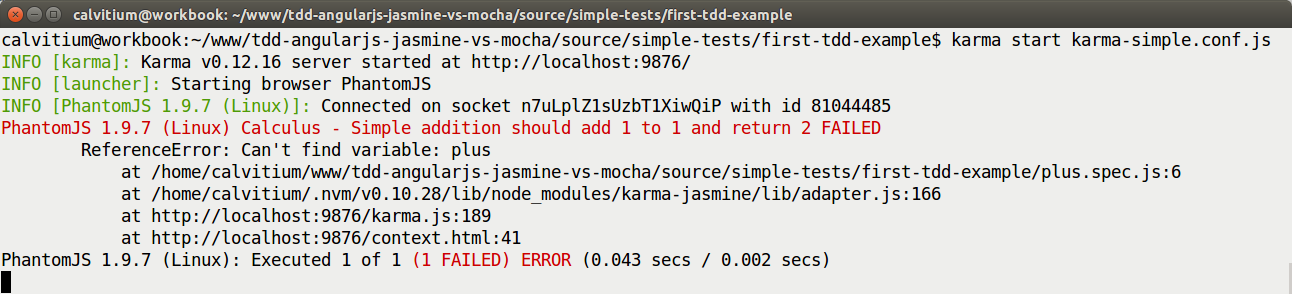
\includegraphics[width=15cm]{images/tdd-simple-step-1-1.png}
  }
  \caption{Terminal Ausgabe des ersten Tests}
  \label{figure:tdd-simple-step-1-1}
\end{figure}

\textbf{Schritt 2: Test bestehen.}\newline
Um diesen Test möglichst schnell dazu zu bringen, grünes Feedback zu geben, wird die einfachste und naivste Implementierung verwendet. Die einfachste Variante bedeutet also, eine Funktion zu definieren, welche zwei Parameter übernimmt und \glqq{2\grqq} zurückgibt (Listing \ref{listing:tdd-simple-addition-implementation}).

\begin{lstlisting}[language=JavaScript, caption=TDD - Calculus - Simple addition - Implementation, label=listing:tdd-simple-addition-implementation]
var plus = function(augend, addend) {
  return 2;
};
\end{lstlisting}

Es existiert hier eine klare, saubere und offensichtliche Lösung und es spricht nichts dagegen, diese hier auch anzuwenden. Um jedoch den dritten Schritt illustrieren zu können, wird hier naiv vorgegangen.\newline
Nach dieser naiven Implementierung ändert sich das Ergebnis des Tests von rot auf grün (siehe Abbildung \ref{figure:tdd-simple-step-1-2}).

\begin{figure}[H]
  \centering
  \fbox{
  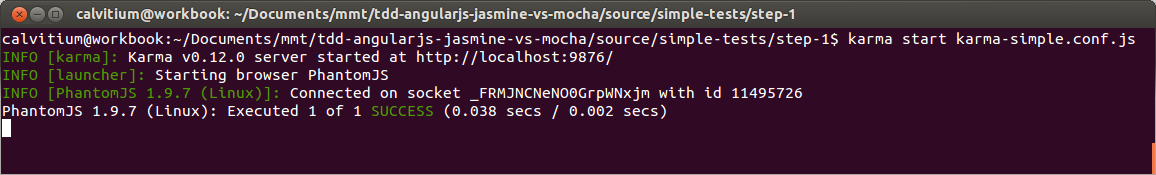
\includegraphics[width=15cm]{images/tdd-simple-step-1-2.png}
  }
  \caption{Terminal Ausgabe des ersten Tests nach naiver Implementierung}
  \label{figure:tdd-simple-step-1-2}
\end{figure}

\textbf{Schritt 3: Es richtig machen.}\newline
Obwohl der Test nun bereits erfolgreich läuft, ist klar, dass diese naive Implementierung nicht korrekt ist. Es handelt sich um eine \glqq{Fake\grqq}-Implementierung. Um nun die richtige Berechnung durchzuführen, wird die Funktion \glqq{plus(arg1, arg2)\grqq} folgendermaßen geändert:

\begin{lstlisting}[language=JavaScript, caption=TDD - Calculus - Simple addition - Refactoring]
var plus = function(augend, addend) {
  return augend+addend;
};
\end{lstlisting}

Nach dem dritten Schritt wird der Test erneut ausgeführt, um zu garantieren, dass das Korrigieren der naiven Implementierung funktioniert. Es wird ein positives Ergebnis erwartet (siehe Abbildung \ref{figure:tdd-simple-step-1-3}).

\begin{figure}[H]
  \centering
  \fbox{
  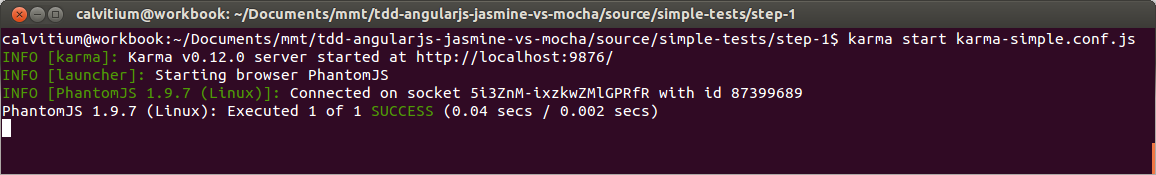
\includegraphics[width=15cm]{images/tdd-simple-step-1-3.png}
  }
  \caption{Terminal Ausgabe des ersten Tests nach Richtigstellung der Implementierung}
  \label{figure:tdd-simple-step-1-3}
\end{figure}

Durch die Anwendung des TDD-Kreislaufs wurde \textit{sauberer} und \textit{funktionierender} Code produziert.

\newpage
\subsection{Test-Driven Development Patterns}
\subsubsection{Red Bar Patterns}

Diese Muster betreffen den ersten Teil des TDD-Kreislaufs: das Test Schreiben.
Konkret behandeln sie die Fragen:
\begin{itemize}
  \item \glqq{Wann\grqq} sollen Tests geschrieben werden?
  \item \glqq{Wo\grqq} sollen Tests geschrieben werden?
  \item \glqq{Wann\grqq} soll mit dem Schreiben von Tests \glqq{aufgehört\grqq} werden?
\end{itemize}

\paragraph{Starter Test}
Mit welchem Test soll begonnen werden?

Eines der Grundkonzepte von TDD besagt, dass die Konzentration immer nur auf dem aktuellen Problem und Test liegen soll. Diesem Konzept steht jedoch die Möglichkeit, mit einem realistischen Test zu starten gegenüber. Bei dem Versuch, einen realistischen Test zu schreiben, wird der Fokus sofort auf einige andere Fragen gelenkt: 
\begin{itemize}
  \item \glqq{Was ist der richtige Input?\grqq}
  \item \glqq{Was ist das richtige Ergebnis?\grqq}
  \item \glqq{Welche Parameter sind notwendig für Lösung des Problems?\grqq}
  \item \glqq{Wohin gehört dieser Test eigentlich?\grqq}
\end{itemize}
Man findet sich bei dem Schreiben realistischer Tests häufig dabei wieder, über viele Probleme und Fragen auf einmal nachzudenken, verliert also den Fokus auf den aktuellen Test des aktuellen Problems.

Ein realistischer Test bedeutet eine Verzögerung des Abstands der \glqq{Rot-Grün-Refactoring\grqq} Zyklen -- diese sollen jedoch möglichst kurz gehalten werden. Der erste Test, also der \glqq{Starter Test\grqq}, soll so trivial wie möglich sein.

\glqq{Start by testing a variant of an operation that doesn't do anything\grqq} \autocite[134]{Beck:2003}.

\paragraph{One Step Test}
Bei TDD handelt es sich um einen Prozess, bei dem in kleinen Schritten Software aus Tests geformt wird. In diesem Prozess ist es notwendig, sich für die Reihenfolge der Test-Schritte (in weiterer Folge auch für die Reihenfolge, in welcher die Komponenten der Software entstehen soll) zu entscheiden.

\cite[134]{Beck:2003} liefert auf die Frage \glqq{Welchen Test sollte ich als nächstes schreiben?\grqq} eine klare Antwort: Es gibt keine.
Die Frage ist hinsichtlich der Anforderungen der Software (beziehungsweise deren Komponenten) sowie der/s Entwicklerin/s zu individuell.
Beck gibt jedoch den Tipp, weder Tests mit einer offensichtlichen Implementierung, noch Tests, welche zu kompliziert erscheinen, zu wählen. Man sollte Schritt für Schritt jene Tests wählen, bei denen man sich am wohlsten fühlt. Sollten nur zu komplizierte Probleme und Tests vorliegen, müssen die Schritte verkleinert und somit das Szenario noch weiter unterteilt werden.

Die Mechanik des \glqq{One Step Tests\grqq} wird von \cite[134]{Beck:2003} mit \glqq{known to unknown\grqq} beschrieben.

\paragraph{Learning Test}

Wie bereits erwähnt, geht es bei TDD nicht nur um eine möglichst hohe Test-Dichte, sondern ebenfalls um andere Faktoren, wie Design, zeitliche Schätzbarkeit, sauberen Code, psychologische Auswirkungen, etc.

Eine weitere Methode TDD einzusetzen, betrifft das Lernen des Umgangs mit einem neuen Appliation Programming Interface (API) oder einer neuen Bibliothek. Wenn man eine neue Bibliothek verwendet, bietet es sich an, für diese Tests zu schreiben, anstatt direkt Implementierungen damit vorzunehmen -- ansonsten sollten keine Tests für externe Software notwendig sein.

\paragraph{Regression Test}
Wenn ein Fehler in einer Applikation auftritt, so ist eine Variante, dieses Problem zu lösen, direkt den Fehler zu finden, zu behen, zu überprüfen und damit den Fehler abzuhaken. Mit dieser Variante gibt es allerdings keine Möglichkeit, zu garantieren, dass dieser Fehler (durch Abhängigkeiten zu anderen Komponenten) nicht erneut auftritt.

Auch TDD kann keine 100\%-ige Fehler-Freiheit garantieren. Sollte ein Problem berichtet werden, ist der erste Schritt, einen neuen Test für dieses Problem zu verfassen. Der Test muss den einfachsten Fall, welcher das Fehlverhalten hervorruft, behandeln. Durch das nachträgliche Absolvieren des TDD-Kreislaufs wird sichergestellt, dass genau dieser Fehler nicht erneut auftritt.

\newpage
\subsubsection{Green Bar Patterns}

Die \glqq{Red Bar Patterns\grqq} helfen dabei, die notwendigen Tests zu verfassen. Die \glqq{Green Bar Patterns\grqq} hingegen geben nun Ansätze, wie die geschriebenen und fehlschlagenden Tests schnellst möglich erfolgreich abgeschlossen werden können.

\paragraph{Fake it ('til you make it)}

Um die Abstände der \glqq{Rot-Grün-Refactoring\grqq} Zyklen so gering wie möglich zu halten, wird immer die einfachste Variante aller möglichen Implementierungen verwendet: Eine Konstante zurückgeben.

Nachdem der Test grün ist, wird Schritt für Schritt die Implementierung richtig gestellt und die Konstante mit Variablen in einen Ausdruck gewandelt. Hier stellt sich jedoch die Frage \glqq{Wieso offensichtlich falschen Code schreiben?\grqq} -- Die Antwort darauf lautet: \glqq{Um den Test schnell erfolgreich laufen zu lassen.\grqq}

Laut \cite[152]{Beck:2003} hat dieses Muster zwei starke Effekte. Wenn der Test grün ist, fühlt man sich sicher. Man kann sich voll und ganz auf das richtige Refactoring konzentrieren. Also einerseits erfüllt \glqq{Fake it\grqq} einen psychologischen Effekt. Andererseits hilft es bei der Abgrenzung von zukünftigen Problemen. Wie schon erwähnt, dient TDD auch dazu, den Fokus und die Konzentration immer bei dem aktuellen Problem zu halten. Als ersten Schritt eine Konstante zurückzugeben, unterstützt die/den EntwicklerIn dabei.

Das folgende Beispiel zeigt das Fake it Pattern anhand einer einfachen Addition von zwei Zahlen. Das Beispiel befindet sich im Verzeichnis \glqq{/source/simple-steps/green-bar-patters/fake-it/\grqq}

\vspace{0.5cm}
\textbf{Schritt 1: Rot}
\begin{lstlisting}[language=JavaScript, caption=TDD - Fake It, label=listing:tdd-fake-it]
// fakeIt.spec.js

describe("Simple calculator", function() {
  it("should add 1 to 1 and return 2", function() {
    expect(sum(1,1)).toEqual(2);
  });
});
\end{lstlisting}
Dieser Test (Listing \ref{listing:tdd-fake-it}) endet natürlich rot, denn die Funktion \glqq{sum\grqq} wurde noch nicht definiert.

\newpage
\textbf{Schritt 2: Grün}
\begin{lstlisting}[language=JavaScript, caption=TDD - Fake It - Implementation, label=listing:tdd-fake-it-implementation]
// fakeIt.js

var sum = function(augend, addend) {
  return 2;
};
\end{lstlisting}

Fake it! -- die einfachste Variante um den geschrieben Test grün abzuschließen, lautet: eine Konstante zurückgeben. Der Test schließt nun positiv ab.

Anmerkung: der vorgehende Schritt wäre gewesen, nur die Funktion \glqq{sum\grqq} zu definieren - um Fake it zu demonstrieren, wurde dieser Schritt übersprungen.

\vspace{0.5cm}
\textbf{Schritt 3: Refactoring} \newline
Im letzten Schritt wird die Duplikation, welche durch Fake it hinzugefügt wurde, entfernt. Es geht nicht um Duplikation innerhalb des Tests oder innerhalb des Produktionscodes, sondern um die Duplikation von Tests und Produktionscode \textit{zusammen}. In Zeile 5 des Tests (Listing \ref{listing:tdd-fake-it}) wird der erwartete Rückgabewert bestimmt -- in diesem Fall die Number \glqq{2\grqq}. In Zeile 4 des Produktionscodes (Listing \ref{listing:tdd-fake-it-implementation}) wird ebenfalls die Number \glqq{2\grqq} verwendet. Diese Duplikation gilt es zu eliminieren.

\begin{lstlisting}[language=JavaScript, , caption=TDD - Fake It - Refactoring]
// fakeIt.js

var sum = function(augend, addend) {
  return augend + addend;
};
\end{lstlisting}

Nach dem Refactoring wird der Test erneut ausgeführt, um sicher zu stellen, dass der Code funktioniert.

Aus diesem Beispiel wird ersichtlich, dass es sich bei \glqq{Duplikation eliminieren\grqq} nicht immer nur um Duplikation innerhalb der Tests oder des Produktionscodes handelt, sondern auch um die Duplikation zwischen Tests und Produktionscode.

\paragraph{Triangulate}

Im Beispiel von Fake it wurde durch das Eliminieren von Duplikation die Implementierung richtig gestellt. Ein anderer Weg, eine richtige Implementierung nach dem Fake it Pattern zu erreichen, ist \glqq{Triangulate\grqq}. Bei Triangulate geht es darum, nicht nur ein mögliches Ergebnis zu testen, sondern zwei oder mehrere Ergebnisse. Durch die genauere Spezifizierung des Tests wird die richtige Implementierung eingegrenzt.

Anhand des folgenden Beispiels wird die Funktionsweise von Triangulate erklärt. Das Beispiel befindet sich im Verzeichnis \glqq{/source/simple-steps/green-bar-patters/triangulate/\grqq}.
Hier wird von Schritt 2 des \glqq{Fake it\grqq} Beispiels (Listing \ref{listing:tdd-fake-it-implementation}) ausgegangen. Es wurde bereits ein Test geschrieben und der Produktionscode dazu mittels Fake it implementiert. Anstatt nun die Duplikation zwischen Tests und Produktionscode zu suchen, wird das Pattern Triangulate angewandt, um die richtige Implementierung zu erreichen.

\vspace{0.5cm}
\textbf{Schritt 3: Triangulate}
\begin{lstlisting}[language=JavaScript, caption=TDD - Triangulate]
// triangulate.spec.js
describe("Simple calculator", function() {
  it("should add 1 to 1 and return 2", function() {
    expect(sum(1,1)).toEqual(2);
  });
  it("should add 1 to 2 and return 3", function() {
    expect(sum(1,2)).toEqual(3);
  });
});
\end{lstlisting}

Es wurde ein weiterer Test hinzugefügt, um die richtige Implementierung einzugrenzen. Da der neue Test fehlschlägt, wird klar, dass die Fake it Implementierung nicht die richtige ist, um das gegebene Problem zu lösen. Nun gäbe es verschiedene Wege, den Test wieder grün abschließen zu können. Man könnte die Implementierung beispielsweise wie folgt ändern:

\begin{lstlisting}[language=JavaScript, caption=TDD - Triangulate - Implementation]
// triangulate.js

var sum = function(augend, addend) {
  if(addend == 2) {
    return 3;
  }
  return 2;
};
\end{lstlisting}

Durch die weitere Anwendung von Triangulate wird die richtige Implementierung weiter eingeschränkt:
\begin{lstlisting}[language=JavaScript, caption=TDD - Triangulate - 2]
// triangulate.spec.js

describe("Simple calculator", function() {
  it("should add 1 to 1 and return 2", function() {
    expect(sum(1,1)).toEqual(2);
  });
  it("should add 1 to 2 and return 3", function() {
    expect(sum(1,2)).toEqual(3);
  });
  it("should add 2 to 1 and return 3", function() {
    expect(sum(2,1)).toEqual(3);
  });
});

\end{lstlisting}
Der Test schlägt fehl und somit ist wieder klar, dass es sich nicht um die korrekte Implementierung für das Problem handelt. Mit Triangulate kann man das Problem so weit einschränken, bis die richtige Lösung ersichtlich wird.
\begin{lstlisting}[language=JavaScript, caption=TDD - Triangulate - Implementation - 2]
// triangulate.js
var sum = function(augend, addend) {
  return augend + addend;
};
\end{lstlisting}

\paragraph{Obvious Implementation}

Wie die bisherigen Beispiele für \glqq{Fake it\grqq} und \glqq{Triangulate\grqq} zeigen, handelt es sich dabei um wirklich kleine Schritte. Speziell anhand dieses Beispiels lässt sich das dritte Green Bar Patterns erklären: \glqq{Obvious Implementation\grqq}.

Wenn eine Operation so einfach ist, wie in dem vorangegangenem Beispiel, spricht nichts dagegen, die offensichtliche Implementierung direkt zu verwenden.
Wenn die Probleme allerdings komplizierter werden, ist es oft schwierig, die Eigenschaften \glqq{sauber\grqq} und \glqq{funktionierend\grqq} gleichzeitig zu erreichen. Außerdem soll der Abstand zwischen den Zyklen möglichst gering gehalten werden, was bei einer offensichtlichen Lösung für ein großes Problem eventuell nicht eingehalten werden kann.

\paragraph{One to many}

Auch bei Operationen welche eine Kollektion von Objekten (beispielsweise ein Array) benötigen gilt: einfach und simpel starten - \glqq{one to many\grqq} \autocite[154]{Beck:2003}.

Zuerst erfolgt die Implementierung mit einem Objekt und erst wenn der Test erfolgreich war, wird Schritt für Schritt die Kollektion übernommen.

Das Beispiel Listing \ref{listing:tdd-one-to-many} soll die Implementierung für \glqq{sum\grqq} erweitern. Es soll möglich sein, nicht nur zwei Zahlen, sondern eine beliebige Anzahl von Zahlen, zu addieren. Das Beispiel befindet sich im Verzeichnis \glqq{/source/simple-tests/green-bar-patterns/one-to-many/\grqq} und geht von der korrekten Implementierung von \glqq{sum\grqq} des Fake it Beispiels aus.

\begin{lstlisting}[language=JavaScript, caption=TDD - One to many, label=listing:tdd-one-to-many]
// oneToMany.spec.js

describe("Simple calculator", function() {
  it("should add 1 to 1 and return 2", function() {
    expect(sum(1,1)).toEqual(2);
  });
});
\end{lstlisting}
\newpage
\begin{lstlisting}[language=JavaScript, caption=TDD - One to many - Implementation]
// oneToMany.js

var sum = function(augend, addend) {
  return augend + addend;
};
\end{lstlisting}

Da mit TDD kein Code geschrieben wird, ohne das ein Test fehlschlägt, wird das neue Problem mit einem Test gestartet.

\begin{lstlisting}[language=JavaScript, caption=TDD - One to many - 2]
// oneToMany.spec.js

describe("Simple calculator", function() {
  it("should add 1 to 1 and return 2", function() {
    expect(sum(1,1)).toEqual(2);
  });

  it("should sum up 1, 1 and 1 and return 3", function() {
    expect(sum([1,1,1])).toEqual(3);
  });
});

\end{lstlisting}

Der erste Test bleibt grün, der neue Test jedoch schlägt fehl. Bei einem roten Test wird implementiert. Hierbei gilt es, Änderungen zu isolieren, dass heißt, die aktuelle Implementierung noch nicht direkt zu ändern, denn der erste Test bestätigt uns, dass diese korrekt funktioniert.

\begin{lstlisting}[language=JavaScript, caption=TDD - One to many - Implementation - 2, label=listing:tdd-one-to-many-implementation-2]
// oneToMany.js

var sum = function(augend, addend) {

  if(augend instanceof Array && typeof(addend) === 'undefined') {
    return 3;
  }

  return augend + addend;
};
\end{lstlisting}

Die Änderung des Produktionscode erfolgte isoliert -- da die aktuelle Implementierung nicht geändert wurde (Listing \ref{listing:tdd-one-to-many-implementation-2}, Zeile 9) -- und wurde mit Fake it implementiert, um schnell in einen grünen Status zu kommen. Da es sich hier um eine offensichtliche Lösung handelt, wird nun nicht mehr trianguliert, sondern direkt die Lösung implementiert.
\newpage
\begin{lstlisting}[language=JavaScript, caption=TDD - One to many - Implementation - 3]
// oneToMany.js

var sum = function(augend, addend) {

  if(augend instanceof Array && typeof(addend) === 'undefined') {
    var sum = 0;
    for(var i = 0; i < augend.length; ++i) {
      sum += augend[i];
    }
    return sum;
  }

  return augend + addend;
};
\end{lstlisting}

Die Änderung wurde isoliert vom Ausgangscode implementiert. Da die Änderung jedoch auch den Ausgangscode ersetzen kann, wird diese nun komplett für die Funktion \glqq{sum\grqq} übernommen werden. Da die neue Implementierung mit einer Array arbeitet und nicht mehr mit zwei Parametern, muss der erste Test ebenfalls angepasst werden.

\begin{lstlisting}[language=JavaScript, caption=TDD - One to many - 3]
// oneToMany.spec.js

describe("Simple calculator", function() {
  it("should add 1 to 1 and return 2", function() {
    expect(sum([1,1])).toEqual(2);
  });
  it("should sum up 1, 1 and 1 and return 3", function() {
    expect(sum([1,1,1])).toEqual(3);
  });
});
\end{lstlisting}

\begin{lstlisting}[language=JavaScript, caption=TDD - One to many - Implementation]
// oneToMany.js

var sum = function(numbersToSumUp) {
    var sumToReturn = 0;
    for(var i = 0; i < numbersToSumUp.length; ++i) {
      sumToReturn += numbersToSumUp[i];
    }
    return sumToReturn;
};
\end{lstlisting}

\newpage
\subsubsection{Mocks, Stubs \& Spies}
In der Entwicklung werden Komponenten mit unterschiedlicher Komplexität verwendet. Es gilt allerdings, alle Komponenten (insbesondere bei TDD) zu testen. Das bedeutet, dass manche Komponenten ressourcen-intensivere Objekte verwenden als andere. Viele ressourcen-intensive Objekte in einem Test zu verwenden, wirkt sich negativ auf die Testdauer aus. Eine längere Testdauer führt dazu, dass diese Tests von EntwicklerInnen tendenziell seltener ausgeführt werden \autocite[4]{Johansen:2011}. Für das Entwickeln mittels TDD bedeutet es längere Rot-Grün-Refactoring Phasen und verzögertes Feedback für die/ den EntwicklerIn.

Um langsame Tests zu vermeiden, werden die ressourcen-intensiven Objekte oft durch \glqq{Fake Objects\grqq}, also gefälschte Objekte, ersetzt. Es gibt einige Varianten, um Objekte für das Testen zu immitieren, die wichtigsten sind:

\begin{itemize}
  \item Mocks
  \item Stubs
  \item Spies
\end{itemize}

Die genannten Varianten verfolgen alle das selbe Ziel - das Immitieren von Objekten - unterscheiden sich allerdings durch die zusätzliche Funktionalität und die Test-Mentalität \autocite{Fowler:Mocks}. Die folgenden Kapitel gehen näher auf jede Variante ein.

\paragraph{Mocks}
\glqq{Mocks\grqq} -- auch \glqq{Mock Objects\grqq} oder \glqq{Pseudo-Objekte\grqq} genannt -- besitzen ein vorprogrammiertes Verhalten, eine vorprogrammierte Erwartung und eine vorprogrammierte Verhaltensüberprüfung \autocite[453]{Johansen:2011}. Darüber hinaus können diese Objekte vor deren Verwendung konfiguriert werden. Mocks werden verwendet, um das \textbf{Verhalten} eines Objektes zu überprüfen. Die Verwendung eines Mock Objektes läuft durch folgende Phasen \autocite[453]{Johansen:2011}:
\begin{enumerate}
  \item \textbf{Konfiguration}: \newline
  Die verschiedenen Stati des Verhaltens werden gesetzt.
  \item \textbf{Ausführung}: \newline
  Das Mock Objekt wird mit der zu testenden Komponente ausgeführt.
  \item \textbf{Verhaltensüberprüfung}: \newline
  Die vorkonfigurierten Stati des ausgeführten Verhaltens werden überprüft.
\end{enumerate}

Ein klassisches Beispiel für ein ressourcen-intensives Objekt, welches durch ein Mock Objekt ersetzt werden kann, ist ein Datenbank-Objekt \autocite[144]{Beck:2003}. Bei der Verwendung eines Datenbank-Objekts kann es zu einer Verzögerung der Tests kommen. Gründe dafür können eine lange Dauer für das Starten der Datenbank oder eventuell ein anderer (entfernter) physischer Standort der Datenbank und somit zusätzliche Netzwerkverzögerung sein. Um diesen Faktoren vorzubeugen, gibt es die Möglichkeit, eine Mock-Datenbank zu verwenden. Die Mock-Datenbank kann vor dem Test konfiguriert werden. Die Konfiguration beinhaltet für eine Mock-Datenbank typischerweise eine erwartete Abfrage (\glqq{expectedQuery\grqq}) und ein erwartetes Ergebnis (\glqq{expectedResult\grqq}). Wird nun im weiteren Testverlauf eine falsche (beziehungsweise nicht erwartete) Abfrage an die Mock-Datenbank geschickt, oder das Ergebnis mit einem nicht erwarteten Wert verglichen, wirft die Mock-Datenbank eine Exception.

Das manuelle Erstellen von Mocks ist nicht so einfach, wie beispielsweise das manuelle Erstellen von Stubs. In der Regel werden also third-party Mocks herangezogen. Die Mocks für JavaScript/AngularJS werden in Kapitel \glqq{AngularJS\grqq} genauer ausgeführt.

\cite[145]{Beck:2003} merkt zu Mocks an, dass man durch deren Verwendung zusätzliche Risiken zu dem betreffenden Projekt hinzufügt. Wenn beispielsweise die extern produzierten Mocks fehlerhaft sind, so können Tests für eine Komponente grün abschließen, welche eigentlich ebenfalls fehlerhaft ist. Vice versa bedeutet dies, dass Tests fehlschlagen können, welche eine einwandfrei funktionierende Komponente betreffen.
Um diese Risiken zu minimieren, schlägt Beck vor, das Verhalten des richtigen Objekts mit jenem des gefälschten Objekts zu vergleichen.

\paragraph{Stubs}
\glqq{Stubs\grqq} ersetzen ebenfalls ressourcen-intensive Objekte durch gefälschte Objekte mit vorprogrammiertem Verhalten. Im Gegensatz zu den Mocks besitzen diese allerdings keine Verhaltensüberprüfung. Stubs geben unabhängig von übergebenen Parametern einen spezifischen vorkonfigurierten Wert zurück, oder werfen bei fehlerhaftem Verhalten eine Exception \autocite[443]{Johansen:2011}. Sie ignorieren darüber hinaus alles, was außerhalb des Tests passiert \autocite{Fowler:Mocks}.

Mit Stubs ist es also prinzipiell nicht möglich, eine sofortige Verhaltensüberprüfung durchzuführen, sondern es wird isoliert der Rückgabewert überprüft. Um das Verhalten im Nachhinein zu überprüfen, können manche Stubs Informationen über die einzelnen Aufrufe der Methoden des Stub Objekts aufzeichnen.

\newpage
\paragraph{Spies}
Die dritte Variante von Fake Objects sind \glqq{Spies\grqq}. Spies -- oder auch Spione -- werden verwendet, um zu überprüfen ob Methoden...
\begin{itemize}
  \item ... aufgerufen oder nicht aufgerufen werden.
  \item ... in der korrekten Reihenfolge aufgerufen werden.
  \item ... die korrekte Anzahl von Aufrufen erfolgt ist.
\end{itemize}

Spies werden oft durch Stubs, welche die Aufrufe aufzeichnen und danach überprüfen, implementiert.

\subsection{Refactoring}
Nachdem die rote sowie grüne Phase des TDD-Kreislauf absolviert wurden, kommt es zu dritten Phase: Dem Refactoring. Da der Fokus dieser Arbeit auf dem Testen liegt, wird dieses Kapitel lediglich einen Überblick über Refactoring geben.

\glqq{Refactoring\grqq} ist eine Änderung einer Software, welche in der internen Struktur gemacht wurde, um diese verständlicher und leichter modifizierbar zu machen, ohne dass nach außen sichtbare Verhalten zu ändern \autocite[53]{Fowler:2012}. Das Verb \glqq{refactor\grqq} bedeutet, Software durch die Anwendung einer Serie von Refactorings umzustrukturieren, ohne das nach außen sichtbare Verhalten zu ändern \autocite[54]{Fowler:2012}.

Refactoring bedeutet laut \cite{Fowler:2012} jedoch nicht nur, den Code aufzuräumen, sondern es ist ebenfalls ein strukturierter Weg, um effizient und kontrolliert sauberen Code zu erhalten. Es hilft dabei Code \glqq{Smells\grqq} zu idenzifieren und zu beseitigen. Die Bezeichnung Code Smells kommt laut \cite{Fowler:2012} von Kent Beck und beschreibt Stellen im Code, welche es zu refactoren gilt. Code-Duplikation, zu lange Methoden oder zu große Klassen sind nur ein kleiner Ausschnitt daraus, was zu Code Smells zählt \autocite[67-88]{Fowler:2012}.

Refactoring bietet nach dem Identifizieren von Code Smells Techniken, um den Code an diesen Stellen zu verbessern. Zu diesen Techniken zählen \glqq{Methode extrahieren/verschieben\grqq}, \glqq{Klasse extrahieren\grqq}, \glqq{Parameter hinzufügen/entfernen\grqq}, etc. Die verschiedenen Code Smells und Möglichkeiten des Refactorings sind zu umfassend für diese Arbeit und werden von \cite{Fowler:2012} ausführlich behandelt.

Viele IDEs helfen EntwicklerInnen beim Refactoring (beispielsweise die Open-Source IDE Eclipse\footnote{http://www.eclipse.org/}) und auch für JavaScript gibt es bereits IDEs, welche einige der Refactoring Techniken (zum Beispiel eine Methode extrahieren oder umbennen) anbieten (beispielsweise WebStorm).

\subsection{Vorteile von TDD}
\label{Vorteile von TDD}
Die bisherigen Kapitel dieser Arbeit erläutern die Prozesse, Funktionsweisen, Auswirkungen sowie Pattern von TDD. Dieses Kapitel fasst die wichtigsten Vorteile von TDD zusammen.
\begin{itemize}
  \item \textbf{Funktionierender Code}\newline
  Durch die hohe Dichte an Tests wird die Fehleranfälligkeit verringert und die Stabilität der geschriebenen Software erhöht. Der TDD Zyklus \glqq{zwingt\grqq} EntwicklerInnen förmlich dazu, anhand von Tests vor der Implementierung darüber nachzudenken.
  \item \textbf{Sauberer Code}\newline
  Durch TDD wird das Refactoring automatisch in den Entwicklungsprozess integriert (siehe Kapitel \glqq{3.4.2 Green Bar Patterns\grqq}). Als Ergebnis erhält man sauberen Code. Durch die zuvor entstandenen Tests wird in diesem Schritt garantiert, dass sich durch das Refactoren keine Bugs einschleichen. Weiters wird durch TDD die Wertschätzung des \glqq{Single Responsibility\grqq} Prinzips und die lose Kopplung der Komponenten gefördert \autocite[30]{Johansen:2011}.
  \item \textbf{Psychologische Effekte}\newline
  Das positive Feedback wirkt sich positiv auf das Stresslevel von EntwicklerInnen aus.
  TDD hilft dabei, sich nur auf das aktuelle Problem zu konzentrieren und sich von zukünftigen Problemen und Entscheidungen abzugrenzen \autocite{Beck:2003}.
  \item \textbf{Dokumentation}\newline
  Mit TDD wird Software aus Tests geformt. Tests wiederum \glqq{erzählen\grqq} eine Geschichte. Sie spiegeln die Anforderungen und die vorgesehen Implementierung einer Komponente wider. Tests können somit auch eine gewisse Dokumentationsfunktion erfüllen und zur besseren Verständnis von Software und einzelnen Komponenten beitragen.
  \item \textbf{Produktivität}\newline
  Das Hauptargument gegen TDD lautet: TDD benötigt Zeit und muss gelernt werden.
  Ist TDD jedoch einmal gelernt und wird regelmäßig angewandt, sorgt es durch alle bisher genannten Vorteile für einen Produktionsschub.
\end{itemize}

\newpage
\section{AngularJS}
\label{AngularJS}
Die Anfänge von AngularJS können laut \cite{Green:2013} bis ins Jahr 2009 zurück verfolgt werden. Anhand eines Projekts namens \glqq{Google Feedback\grqq} wollte der Schaffer der Open-Source Bibliothek -- Misko Hevery -- diese seinen MitarbeiterInnen vorstellen. Er behauptete das gesamte Projekt, welches bis zu diesem Zeitpunkt aus circa 17.000 Zeilen Frontend-Code bestand, innerhalb von zwei Wochen neu schreiben zu können. Nach drei Wochen und 1.500 Zeilen Code war Hevery fertig.

Nach diesem Erfolg wurde ein Team rund um das Projekt Angular gebildet, um Heverys Konzepte umzusetzen und zu verbessern. Daraus entstand das heute bekannte JavaScript MVC/W Framework AngularJS. Entwickelt wurde und wird es sowohl von Google Teams als auch von der Open-Source Community.

Dieses Kapitel stellt die Konzepte, auf welchen Angular beruht, und die Anatomie von Angular vor.

\subsection{Konzepte}
Die folgenden Konzepte wurden von erfolgreichen Vorbildern aus anderen Frameworks auf die Verwendung mit HTML, Browsern und anderen Web-Standards übertragen. Sie beziehen sich auf \cite[2-6]{Green:2013}.

\subsubsection{Client-Side Templates}
Viele Web-Applikationen erstellen das anzuzeigende HTML Dokument durch vorgefertige Templates, welche am Server mit zusätzlichen Daten befüllt, und anschließend an den Client zur Anzeige im Browser geschickt werden.

Angular unterscheidet sich von dieser Herangehensweise. Templates und Daten werden an den Browser geschickt und erst dort zusammengeführt und angezeigt. Der Server dient somit nur mehr als statischer Ressourcen Lieferant der Templates und dafür, die für das Befüllen des Templates benötigten Daten zu liefern.

\subsubsection{Model View Controller/Whatever (MVC/W)}
Die Kern-Idee von MVC ist es, eine klare und saubere Trennung der Daten (der \textit{Models}) der Applikationslogik (der \textit{Controllers}) sowie der Präsentation (der \textit{Views}) zu erreichen. Die View erhält die anzuzeigenden Daten vom Model und präsentiert diese. Bei Interaktionen durch BenutzerInnen (zum Beispiel durch Klicks) antwortet der Controller, indem er das Model ändert. Das Model wiederum benachrichtigt die View, dass Änderungen vorliegen.

\newpage
Für Angular bedeutet dies:
\begin{enumerate}
  \item Das DOM ist die \textit{View}.
  \item JavaScript Klassen sind die \textit{Controller}.
  \item Die \textit{Model-Daten} werden in JavaScript Objekt-Eigenschaften gespeichert.
\end{enumerate}

Einige Gründe für die Verwendung von MVC-Frameworks sind:
\begin{enumerate}
  \item Eine organisierte und klare Struktur.
  \item Die Zusammenarbeit durch viele beitragende MitarbeiterInnen wird vereinfacht, da die Applikation Richtlinien eines bekannten Patterns folgt.
  \item MVC hilft eine Applikation leichter zu erweitern, zu warten und zu testen.
\end{enumerate}

Laut \cite[12]{Kozlowski:2013} ist das Problem mit Frameworks, welche das MVC-Pattern verwenden, jedoch, dass es kein sehr präzises Pattern ist, sondern nur gewisse Rahmenbedingungen auf einer sehr hohen Ebene definiert.

AngularJS verfolgt laut \cite[13]{Kozlowski:2013} einen \glqq{pragmatischeren Ansatz\grqq} und befolgt das \glqq{MVW - Model-View-Whatever\grqq} Pattern -- mit \glqq{Whatever\grqq} ist gemeint: \glqq{whatever works for you\grqq} \autocite{Angular:GooglePlus}.

\subsubsection{Data-Binding}
In der klassischen Web Entwicklung war es üblich ein \glqq{User-Interace (UI)\grqq} zu erstellen, indem Daten und HTML am Server verschmolzen und abschließend an den Browser zur Darstellung ausgeliefert werden. So wurde das UI den NutzerInnen präsentiert. Das \glqq{Asynchronous JavaScript and XML\grqq} (AJAX) Konzept erweitert dies und ermöglicht es, nur einzelne Teile des UIs vom Client aus zu aktualisieren. Neue Daten können vom Server beantragt und anschließend damit das UI durch DOM-Manipulation aktualisiert werden.

Diese Methode, um Daten zu aktualisieren, ist durchaus gängig, birgt aber folgende Problematik: Wenn neue Daten angefordert werden, muss sicher gestellt werden, dass die Daten in den korrekten Status für das UI (die Präsentation) sowie für die betreffenden JavaScript Objekt-Eigenschaften gesetzt werden.

Angular löst dieses Problem durch \glqq{(Two-way) Data-Binding\grqq}. Im UI wird definiert, welche Teile zu welchen JavaScript Objekt.Eigenschaften gehören. Ändern sich nun die Daten an einer Stelle -- egal ob im UI oder in der Objekt-Eigenschaft -- so wird automatisch synchronisiert (deshalb auch \glqq{Two-way\grqq}). Dadurch werden DOM-Zugriffe und Event-Handler wie beispielsweise \glqq{onChange()\grqq} eliminiert. Werden neue Daten von Server angefragt, so müssen diese lediglich in die betreffende JavaScript Objekt-Eigenschaft gesetzt werden und das Data-Binding sorgt dafür, dass das UI dementsprechend synchronisiert wird.

\subsubsection{Dependency Injection}
Angulars Dependency Injection System folgt dem Design Pattern \glqq{Law of Demeter\grqq}, welches auch unter \glqq{Principle of least Knowledge\grqq} bekannt ist. Es müssen keine Abhängigkeiten erstellt werden (wie zum Beispiel \glqq{Klasse foo benötigt Abhängigkeiten zu den Modulen bar und foobar\grqq}), sondern die Klassen fragen direkt nach den Modulen, welche sie benötigen.

Zur Illustration: In jedem Controller existiert ein \glqq{\$scope\grqq}-Objekt (siehe Kapitel \glqq{4.2.1 \$scope\grqq}), welches für das Two-way Data-Binding zuständig ist. Dieses Objekt muss nicht von EntwicklerInnen erstellt werden, es wird dem Controller nur als Argument übergeben. So wird keine Abhängigkeit erstellt, sondern viel mehr nach dem \$scope-Objekt gefragt. Dadurch wird garantiert, dass sich der Controller um nichts anderes (zum Beispiel Data-Binding) als seine Zuständigkeiten kümmern muss (Principle of least Knowledge).

\subsubsection{Directives}
Zur Zeit wird am Standard für \glqq{Web-Components\grqq} gearbeitet \autocite{Glazkov:13:IWC}. Eine Komponente von Web-Components ist \glqq{Custom-Elements\grqq}. Es handelt sich dabei unter anderem um eigene HTML-Elemente beziehungsweise eigene HTML-Templates.

Angular ermöglicht es bereits jetzt, eigene Elemente beziehungsweise eigene HTML-Templates zu erstellen -- mit Directives. Angular besitzt viele Directives, um das Gestalten des UIs zu vereinfachen.

\subsection{Komponenten}
\subsubsection{\$scope}
In jeder Angular Applikation existiert ein \$rootScope Objekt. Scopes sind hierarchisch aufgebaut und der \$rootScope ist der root-Knoten der Hierarchie. Alle weiteren erstellten Scopes sind \glqq{child\grqq}-Scopes. Diese können manuell erstellt werden (\$rootScope.\$new()), dies übernimmt allerdings Angular automatisch, wenn ein neuer Controller erstellt wird.

Ein Scope Objekt ist ein Objekt, welches auf ein Applikations-Model referenziert. Es wird in der Angular Dokumentation als \glqq{der Kleber zwischen einem Controller und einer View\grqq} \autocite[Scopes]{Angular:DevGuide} bezeichnet. Das Scope Objekt trägt einerseits Sorge dafür, dass Änderungen am Applikations-Model an alle beteiligten Views und/oder Controller propagiert werden, und andererseits, dass alle Änderungen überwacht werden (Two-Way Data-Binding).

Diese Aktionen (propagieren und überwachen) können auch manuell ausgeführt werden:
\begin{itemize}
  \item \$scope.\$apply() propagiert Änderungen des Applikations-Models
  \item \$scope.\$watch() überwacht Änderungen des Applikations-Models
\end{itemize}

\subsubsection{Controller}
Ein Angular Controller ist eine JavaScript Konstruktor Funktion, welche ein Angular Scope Objekt als Argument erwartet. Ein Controller kann manuell erstellt werden oder durch Angular Mark-Up an die DOM angehängt werden (<div ng-controller='FooCtrl'></div>). Bei der zweiten Variante wird automatisch ein Child-Scope für diesen Controller erstellt.

Controller sollen für folgende Aktionen verwendet, beziehungsweise nicht verwendet werden \autocite[Controllers]{Angular:DevGuide}:

Controller sollen verwendet werden, um...
\begin{itemize}
  \item ... den initialen Status eines Models des Scopes zu setzen.
  \item ... ein gewisses Verhalten des Scopes zu definieren (beispielsweise um auf Aktionen einer/s NutzerIn reagieren zu können)
\end{itemize}

Controller sollen jedoch ausdrücklich nicht verwendet werden (Seperation of Concerns), um...
\begin{itemize}
  \item ... die DOM zu manipulieren (für DOM-Manipulationen sind entweder Angulars Data-Binding oder Angular Directives zuständig).
  \item ... NutzerInnen-Eingaben zu formatieren (dafür sind Angular Form Controls \autocite[Forms]{Angular:DevGuide} zuständig).
  \item ... Ausgaben zu filtern (um Ausgaben zu filtern sollen Angular Filters verwendet werden).
  \item ... Code oder Objekt-Stati mit anderen Controllern zu teilen (Angular Services sind für diese Zwecke geeignet).
\end{itemize}

\paragraph{Das Testen eines Angular Controllers}
Um einen Controller testen zu können, muss dieser manuell erstellt werden. Dafür kann der Angular Service \glqq{\$controller\grqq} verwendet werden \autocite[\$controller]{Angular:APIRef}. Bei der Erstellung muss darauf geachtet werden, dass alle notwendigen Parameter (zum Beispiel ein Scope Objekt oder ein benötigter Service) übergeben werden.

\subsubsection{Filter}
Angular Filter sind für die korrekte Formatierung einer Ausgabe zuständig. Sie können entweder direkt in einer View verwendet werden, oder von Controllern, Services und Directives instanziiert werden (das jeweilige Modul erhält den Filter durch Dependency Injection).

\newpage
Angular wird bereits mit einigen nützlichen Filtern ausgeliefert. Beispielsweise der \glqq{date\grqq}-Filter \autocite[Filter/Date]{Angular:APIRef}:

\begin{lstlisting}[language=JavaScript, caption=AngularJS - Date-Filter]

<!-- formats a JavaScript date object to a human readable date -->
{{myDate | filter: 'MM/dd/yyyy'}}

\end{lstlisting}

\subsubsection{Services}
Ein Angular Service wird verwendet, um Code oder verschiedene Stati über eine Angular Applikation teilen zu können. Sie werden über Angulars Dependency Injection instanziiert.

Folgendes Beispiel verdeutlicht die Funktionsweise und Verwendung von Services:

Controller \glqq{FooCtrl\grqq} und Controller \glqq{BarCtrl\grqq} sind beide abhängig von dem Status des Models \glqq{FooBar\grqq}. Es wird ein Service \glqq{FooBarService\grqq} erstellt, um den Status teilen zu können. Die Controller verwenden den Service via Dependency Injection:

\begin{lstlisting}[language=JavaScript, caption=AngularJS - Services]

angular.module('App', []).
  service('FooBarService', function(FooBarService) {
    this.fooBar = false;

    this.setFooBar = function(state) {
      this.fooBar = state;
    }
  }).
  controller('FooCtrl', function(FooCtrl, FooBarService) {
    $scope.fooBar = FooBarService.fooBar;
  }).
  controller('BarCtrl', function(BarCtrl, FooBarService) {
    $scope.fooBar = FooBarService.fooBar;
  });

\end{lstlisting}

Wenn nun der \glqq{FooCtrl\grqq} Controller \glqq{FooBarService.setFooBar(true)\grqq} aufruft, so wird automatisch der \$scope des \glqq{BarCtrl\grqq} Controllers aktualisiert.

Services sind \autocite[Services]{Angular:DevGuide}...
\begin{itemize}
  \item \glqq{träge\grqq} (lazily) instanziiert -- Angular instanziiert einen Service nur dann, wenn eine Komponente diesen via Dependency Injection erfordert.
  \item Singletons -- jede Komponente, welche den Service verwendet, erhält eine Referenz zu einer einzigen Instanz des Service.
\end{itemize}

\newpage
Angular \glqq{Services\grqq} können in drei verschiedene Typen von Services unterteilt werden:
\begin{itemize}
  \item Services
  \item Factories
  \item Providers
\end{itemize}

Die Typen unterscheiden sich in folgenden Eigenschaften:
\begin{center}
  \begin{table}[h]
    \begin{tabular}{ p{9cm} | l | l | l}
    \textbf{Eigenschaft} & \textbf{Factory} & \textbf{Service} & \textbf{Provider} \\ \hline
    verwendet \glqq{type-friendly\grqq} Injection & Nein & Ja & Nein \\ \hline
    verfügbar während der config-Phase & Nein & Nein & Ja \\ \hline
    kann primitive JavaScript Typen und Funktionen erstellen & Ja & Nein & Ja \\
    \end{tabular}
    \caption[Unterschiede von AngularJS Services]{Tabelle entnommen aus \cite[Services]{Angular:DevGuide} }
  \end{table}
\end{center}

Aufgrund dieser Unterschiede, werden Services verwendet, um Objekte eines BenutzerInnen-definierten Typs zu erstellen. Factories werden hingegen verwendet, um primitive JavaScript Typen und Funktionen zu erstellen. Wenn der Service global und während der Konfigurationsphase modifizierbar sein soll, werden Providers verwendet. Die Konfigurationsphase findet statt, bevor die die AngularJS Applikation gestartet wird.

\paragraph{Das Testen eines Angular Services}
Um einen Service in einem Test zu instanziieren zu können, muss die Dependency Injection manuell durchgeführt werden. Um dies zu erreichen, wird der Angular Service \glqq{\$injector\grqq} verwendet \autocite[\$injector]{Angular:APIRef}.

\newpage
\subsection{Zusätzliche relevante AngularJS Komponenten}
\begin{itemize}
  \item \textbf{\$route}...\linebreak
      ... ist zuständig für das Routing einer Angular Applikation \autocite[\$route]{Angular:APIRef}. \$route verlinkt eine Route mit einer View und einem Controller. Es kann mit Hilfe des \$routeProviders während der config-Phase konfiguriert werden:

      \begin{lstlisting}[language=JavaScript, caption=AngularJS - {\$}route]
angular.module('App', []).config( function($routeProvider) {
  $routeProvider.when('/foo', {
    templateUrl: 'foo_template',
    controller: 'FooCtrl'
  });
});
      \end{lstlisting}

  \item \textbf{\$http}...\linebreak
      ... ist ein \glqq{... Kern-Angular Service, welcher die Kommunikation mit entfernten HTTP Servern erleichtert... \grqq} \autocite[\$http]{Angular:APIRef}. Der Service nimmt als Argument ein Objekt entgegen, welches alle Informationen über den anstehenden HTTP-Request beinhaltet und liefert ein JavaScript Promise-Objekt zurück. Das Promise-Objekt verfügt über die HTTP-spezifischen Methoden \glqq{success()\grqq} und \glqq{error()\grqq}.

      \begin{lstlisting}[language=JavaScript, caption=AngularJS - {\$}http]
$http({method: 'GET', url: '/foo/bar'})
  .success( function(data) {
  })
  .error( function(data) {
  });
      \end{lstlisting}

      \paragraph{Das Testen des \$http-Services}
      Da beim Testen kein tatsächlicher HTTP-Request abgesetzt werden soll, wird Angular mit einem Mock \glqq{\$httpBackend\grqq} ausgeliefert \autocite[ngMock/service/\$httpBackend]{Angular:APIRef}. Dieser kann in der Test-Phase so konfiguriert werden, dass er einen spezifischen Request erwartet und einen definierten Response zurückliefert. Wenn ein Request abgesetzt wird, welcher nicht vom \$httpBackend-Mock erwartet wird, so kommt es zu einem fehlgeschlagenen Test. Wenn der erwartete Request abgesetzt wurde, wird vom Mock der definierte Response zurückgegeben und dieser kann im Test inspiziert werden.

  \newpage
  \item \textbf{\$resource}...\linebreak
      ... ist eine \glqq{Factory, welche ein resource-Objekt erstellt und es gestattet, einfach mit einem RESTful Server zu interagieren\grqq} \autocite[\$resource]{Angular:APIRef}.

      \begin{lstlisting}[language=JavaScript, caption=AngularJS - {\$resource}]
var Foo = $resource('/foo/:fooId', {fooId: '@id'});

Foo.query()             // GET request to '/foo'
Foo.save({})            // POST request to 'foo'
Foo.get({fooId: 42})    // GET request to '/foo/42'
Foo.delete({fooId: 42}) // DELETE request to '/foo/42'
      \end{lstlisting}

\end{itemize}

\newpage
\section{Testing Frameworks}

\subsection{Jasmine}
Jasmine ist ein Javascript Testing Framework, welches notwendige Funktionen wie Assertions, Matchers, Mocks und Spies anbietet. Es wurde prinzipiell für Behaviour-driven Development (BDD) entworfen. BDD ist ein TDD sehr ähnlicher Entwicklungsprozess \autocite[34]{Johansen:2011}. Bei BDD wird der Fokus auf ein gemeinsam genutztes Vokabular und auf User-Stories gesetzt.

Jasmine verwendet die \glqq{expect\grqq}-Schreibweise für Tests (eine genauere Beschreibung von expect folgt in den nachfolgenden Kapiteln). Im Idealfall lautet ein Testfall bei BDD genau gleich wie eine User-Story, deshalb ist die expect-Schreibweise auch typisch für BDD. Es kann aber selbstverständlich auch für konventionelles Testen und für TDD verwendet werden. Auf der AngularJS Website wird für Test-Beispielen Jasmine verwendet \autocite[Unit Testing]{Angular:DevGuide}.

\subsubsection{Keywords in Jasmine}
Die folgenden Keywords beziehen sich auf \cite[5-8]{Hahn:2013}.
\begin{itemize}
  \item \textbf{describe}:\newline
        Mit \glqq{describe\grqq} wird in Jasmine eine neue Test \glqq{Suite\grqq} erstellt. Eine \glqq{Suite\grqq} ist eine Sammlung von Test-Spezifikationen. \glqq{describe\grqq} beschreibt die Suite in natürlicher Sprache.
\begin{lstlisting}[language=JavaScript]
  describe('What the following test-specifications are about',
    function() {
    ...
  });
\end{lstlisting}
  \item \textbf{it}:\newline
        Der \glqq{it\grqq}-Block befindet sich innerhalb der anonymen Funktion, welche describe übergeben wird. Er versteht sich als Spezifikation. In einer Suite können sich mehrere \glqq{it\grqq}-Blöcke befinden. Ebenso wie bei describe wird die it-Funktion mit natürlicher Sprache beschrieben und eine anonyme Funktion wird ihr mitgegeben.
\begin{lstlisting}[language=JavaScript]
  describe('What the following test-specifications are about.',
    function() {
    it('specifies what the following tests are about.',
      function() {
      ...
    });
  });
\end{lstlisting}
  \item \textbf{expect}:\newline
        Das \glqq{expect\grqq}-Keyword spiegelt den eigentlichen Test wider. Man erwartet ein bestimmtes Ergebnis. Wenn das erwartete Ergebnis eintritt, gilt der Test als bestanden, oder auch als \glqq{grün\grqq}. Sollte dies jedoch nicht der Fall sein, so ist der Test nicht bestanden und wird als \glqq{rot\grqq} bezeichnet. Tests, welche sich in der selben Spezifikation jedoch nach dem fehlgeschlagenem Test befinden, werden nicht mehr ausgeführt.
\begin{lstlisting}[language=JavaScript]
  describe('What the following test-specifications are about.',
    function() {
    it('specifies what the following tests are about.',
      function() {
      expect(true).toEqual(true);    // success
      expect(false).toEqual(true);   // failure
      expect(false).toEqual(false);  // not executed
    });
  });
\end{lstlisting}

\end{itemize}

\subsubsection{Matcher}
\glqq{Matcher\grqq} sind Funktionen, welche zwei Ausdrücke miteinander vergleichen. Das Ergebnis des Vergleichs führt entweder zu einem positivem Test oder bei einem negativem Test zum Abbruch der aktuellen Spezifikation. Jasmine wird bereits mit vielen nützlichen Matcher ausgeliefert und ermöglicht auch das Schreiben von benutzerdefinierten Matcher.

Folgende Matcher sind standardmäßig vorhanden:

\begin{itemize}
  \item \textbf{toEqual} überprüft die \glqq{Gleichheit\grqq} zweier Ausdrücke. Hier findet jedoch keine Identitätsüberprüfung statt (siehe \glqq{toBe\grqq}).

  \item \textbf{toBe} verhält sich ähnlich wie toEqual, mit dem Unterschied der Identitätsüberprüfung. toEqual ist Jasmines Äquivalent zu Javascripts \glqq{==\grqq} Operators, wobei toBe \glqq{===\grqq} entspricht. Da sich toBe auf den \glqq{===\grqq} Operator stützt, garantiert dieser Matcher \textit{nicht} die Identitätsgleichheit bei primitiven Javascript Typen - also nicht bei Numbers, Booleans und Strings. Der \glqq{===\grqq} Operator sieht diese Primitive als idente Entitäten an \autocite[16]{Hahn:2013}.

  \item \textbf{toBeTruthy, toBeFalsy}\newline
  toBeTruthy evaluiert einen Ausdruck auf \glqq{true\grqq} und toBeFalsy auf \glqq{false\grqq}. Genau wie auch in Javascript entsprechen true und false nicht nur den gleichnamigen boolschen Ausdrücken. Als true gelten beispielsweise auch "'Foo"' oder \{\}. Um sicher zu gehen, was nun true und was false ist, ist es einfacher darüber nachzudenken, was in Javascript false ist, denn \glqq{\textit{alles, was nicht false ist, ist true.}\grqq} \autocite[17]{Hahn:2013}.

  \newpage
  False ist:
    \begin{itemize}
      \item false
      \item 0
      \item "'"'
      \item undefined
      \item null
      \item NaN (Not a Number, zum Beispiel die Division durch 0)
    \end{itemize}

  \item \textbf{not} ist eine einfache Verneinung und wird vor einem weiteren Matcher aufgerufen.
  \begin{lstlisting}[language=JavaScript]
    expect(true).not.toBeFalsy(); // success
  \end{lstlisting}

  \item \textbf{toBeDefined, toBeUndefined} überprüfen ob Objekte definiert sind oder nicht. Sie halten sich dabei an den in ECMA-Script definierten Richtlinien für \glqq{defined\grqq} und \glqq{undefined\grqq} (\textit{http://www.ecma-international.org/ecma-262/5.1/}).

  Wichtig: Wenn eine Variable nicht deklariert wurde, so wird eine \glqq{ReferenceError\grqq}-Exception geworfen. Alle Variablen, unabhängig ob definiert oder nicht, müssen deklariert werden.

  \item \textbf{toBeNull} überprüft, ob ein Ausdruck \glqq{null\grqq} ist.

  \item \textbf{toBeNaN} überprüft, ob ein Ausdruck NaN, also Not a Number ist.
  Es gibt bereits eine eigene \glqq{isNaN\grqq} Funktion von Javascript. Diese evaluiert allerdings einige nicht-nummerische Typen als NaN (Strings, Objekte, Arrays). Jasmines toBeNaN evaluiert nur auf den Wert NaN.

  \item \textbf{toBeGreatherThan, toBeLessThan} überprüfen, ob ein Ausdruck größer, beziehungsweise kleiner als ein anderer Ausdruck ist. Das funktioniert für nummerische Typen und auch für Strings.

  \item \textbf{toBeCloseTo} überprüft, ob ein Ausdruck \glqq{nahe\grqq} einem zweiten ist. Die Nähe wird durch Dezimalstellen definiert. Die Dezimalstelle ist das zweite Argument von toBeCloseTo. Die genaue Funktionsweise von toBeCloseTo wird im Kapitel \glqq{Custom Matcher\grqq} illustriert.

  \item \textbf{toMatch} überprüft, ob ein Ausdruck mit einer übergebenen RegularExpression übereinstimmt.

  \item \textbf{toThrow} evaluiert, ob ein Ausdruck eine Exception wirft.

  \item \textbf{jasmine.any} ermöglicht es, den Typ eines Objekts zu überprüfen - ähnlich wie JavaScripts instanceof Operator.


\end{itemize}

\paragraph{Custom Matcher}
Die bereits mitgelieferten Matcher von Jasmine sind sehr nützlich, decken jedoch nicht alle denkbaren Vergleiche ab. Aus diesem Grund gibt es mit Jasmine die Möglichkeit, eigene Matcher zu definieren. Die Definition dieser Matcher muss vor dem it-Block, vor welchem sie verwendet werden sollen, erfolgen.

Dies kann beispielsweise wie folgt implementiert werden.

\begin{lstlisting}[language=JavaScript]
describe('My test-suite' function() {

  beforeEach( function() {
    this.addMatchers({
      matchFn: function() {
        this.message = function() {
          return 'Error-message, input: ' + this.actual;
        }
        return true;
      };
    });
  });

  it('My test-spec', function() {
    expect(true).matchFn(); // success
  });

});
\end{lstlisting}

Custom Matcher bestehen aus drei wichtigen Teilen:
\begin{itemize}
  \item \textbf{this.message}: \newline
  this.message wird ausgeführt, wenn der Matcher fehlschlägt. Hier ist also eine Fehlermeldung mit dem erwarteten und dem richtigen Ergebnis sinnvoll.
  \item \textbf{this.actual}: \newline
  this.actual ist jener Wert, welcher der vorhergehenden expect-Funktion übergeben wurde.
  \item \textbf{return expression}: \newline
  In der return Anweisung wird nun der eigentliche Vergleich ausgeführt. Wenn beispielsweise der Matcher \glqq{toBeGreatherThanTen\grqq} implementiert werden soll, so wäre die return Anweisung:
\begin{lstlisting}[language=JavaScript]
return this.actual > 10;
\end{lstlisting}

\end{itemize}


Bei den bisherigen Matchern war die Funktionalität oft einfach durch die Namensgebung erkennbar. Laut \cite[21]{Hahn:2013} ist jedoch bei einem Matcher nicht auf den ersten Blick erkennbar, was dieser vergleichen/matchen soll.

\newpage
\begin{lstlisting}[language=JavaScript]
expect(MATH.PI).toBeCloseTo(3.1, 1); // success
\end{lstlisting}

Anhand der Erläuterung in Kapitel \textit{toBeGreatherThan, toBeLessThan, toBeCloseTo} wird klar, dass das zweite Argument von toBeCloseTo -- die Dezimalstelle auf welche die zwei Werte verglichen werden sollen -- bestimmt.

\begin{lstlisting}[language=JavaScript]
expect(Math.PI).toBeCloseTo(3.14, 2); // success: 3.14 == 3.14
\end{lstlisting}

\cite[21]{Hahn:2013} schlägt anhand des folgenden Custom Matchers eine weitere mögliche Implementierung (welche laut ihm toBeCloseTo ersetzen könnte) vor:

\begin{lstlisting}[language=JavaScript]

  describe('...', function() {

    beforeEach( function() {

      this.addMatchers({
        toBeWithinOf: function(distance, base) {

          this.message = function() {
            var lower = base - distance;
            var upper = base + distance;
            return 'Expected ' + this.actual + ' to be between ' +
              lower + ' and ' + upper + ' (inclusive).';
          }

          return Math.abs(this.actual - base) <= distance;

        }
      });

    });

    it('should report, that 6 is within of 4 and 8 (inclusive)', function() {
      expect(6).toBeWithinOf(4, 8);
    });

  });

\end{lstlisting}

\subsubsection{Weitere Jasmine Features}

\begin{itemize}
  \item \textbf{Nested Suites}: \newline
  Durch TDD werden in kurzer Zeit viele Tests geschrieben. Wenn nun eine größere Komponente zum Beispiel 20-30 Tests benötigt, so kann man hier eventuell die Übersicht über die Struktur und Logik der Komponente verlieren (da die Tests die Komponente beschreiben). Eine Geschichte besitzt ebenfalls eine Struktur, welche dabei hilft, diese besser zu verstehen. Tests erzählen im besten Fall eine Geschichte über die Komponente \autocite[11]{Beck:2003}.

  Um die Tests nach der richtigen Logik gliedern zu können, ist es mit Jasmine möglich, sogenannte \glqq{Nested Test-Suites\grqq}, also \glqq{verschachtelte Test-Sammlungen\grqq}, zu erstellen.

  \item \textbf{Specs und Suites überspringen}: \newline
  \textbf{Achtung:} Das Überspringen von Test-Specs oder gar ganzen Test-Suites, spricht ausdrücklich gegen die Konventionen des TDD-Zyklus \autocite{Beck:2003}.

  Da Jasmine jedoch kein TDD-Framework ist, ist es jedoch mit sehr einfachen Mitteln möglich Specs oder Suites zu überspringen. Durch das Voranstellen eines \glqq{x\grqq} vor die Keywords describe oder it werden diese einfach ausgelassen.

  \item \textbf{beforeEach} und \textbf{afterEach}: \newline
  Mit \glqq{beforeEach\grqq} und \glqq{afterEach\grqq} kann eine anonyme Funktion vor und nach jedem it-Block oder vor und nach jeder Nested Suite ausgeführt werden. Dies ist nützlich, um (Mock) Objekte, welche von mehreren Spezifikationen verwendet werden, vorzubereiten oder nach deren Verwendung zurückzusetzen.

  \begin{lstlisting}[language=JavaScript]
beforeEach( function() {...});
...
afterEach( function() {...});

  \end{lstlisting}

  Wie bereits in vorhergehenden Kapiteln beschrieben, sollen alle Tests isoliert ablaufen und kein Test soll von einem anderen abhängig sein. Wenn nun ein vorbereitetes Objekt von einem Test verwendet und verändert wird, so ist es wichtig, dieses auch wieder in den richtigen Ausgangsstatus zurückzusetzen. Dafür kann afterEach verwendet werden. afterEach wird nach jeder Spezifikation oder Nested Test Suite in der jeweiligen (Nested) Test Suite ausgeführt.

\end{itemize}

\subsubsection{Spies}
Alle bisherigen Tests betrafen die Vergleiche von mehreren Ausdrücken, es gab jedoch keine Möglichkeit, das Verhalten von Funktionen oder Objekten zu inspizieren. Um das zu erreichen, liefert Jasmine Spies mit. Wie bereits im Kapitel \glqq{Mocks, Stubs \& Spies\grqq} erläutert, handelt es sich dabei um ein Fake Objekt, welches das echte Objekt ersetzt. Aufrufe auf das Fake Objekt werden aufgezeichnet und können am Ende inspiziert werden. Die nachfolgenden Beispiele beziehen sich großteils auf \cite{Jasmine}.

\begin{itemize}
  \item \textbf{spyOn}: \newline
  Um das gewünschte Objekt oder die gewünschte Funktion durch einen Spy zu ersetzen, wird \glqq{spyOn\grqq} verwendet. Die Aufrufe auf den Spy werden mit \glqq{toHaveBeenCalled()\grqq} und \glqq{toHaveBeenCalledWith(args)\grqq} inspiziert.

  In dem folgenden Beispiel wird ein echtes Objekt erstellt und der Spy installiert. In der Testspezifikation werden dann die Aufrufe auf den Spy inspiziert.

  \begin{lstlisting}[language=JavaScript]
describe("A spy", function() {
  var foo = {
    setBar: function(value) {}
  };
    
  it("tracks that the spy was called", function() {
    spyOn(foo, 'setBar');

    foo.setBar(123);
    foo.setBar(456, 'another param');

    expect(foo.setBar).toHaveBeenCalled();
    expect(foo.setBar).toHaveBeenCalledWith(123);
    expect(foo.setBar).toHaveBeenCalledWith(456, 'another param');
  });

});
  \end{lstlisting}

  \item \textbf{and.callThrough}: \newline
  Da Spies die echte Implementierung des Objekts ersetzen, ist es nach der Installation eines Spies nicht mehr möglich, den Ergebnis-Status des Objekts zu ermitteln. Bei Jasmine gibt es allerdings die Funktion \glqq{and.callThrough\grqq}. Diese zeichnet wie auch normale Spies die Aufrufe auf und leitet diese zusätzlich an die echte Implementierung weiter. Hier wird das Fake Objekt also nicht mehr verwendet, um ein ressourcen-intensives Objekt zu ersetzen. Es wird stattdessen verwendet, um das Verhalten aufzuzeichnen und dieses sowie das Endergebenis des echten Objekts mit gewissen Erwartungen zu vergleichen.

  \item \textbf{and.returnValue}: \newline
  Mit \glqq{and.returnValue\grqq} kann sichergestellt werden, dass ein spezifischer Wert zurückgegeben wird. Dies kann beispielsweise hilfreich sein, um eine Komponente mit falschen Eingaben zu testen.

  \item \textbf{and.callFake}: \newline
  Mit einem Spy kann zusätzlich eine Fake Funktion angehängt werden. Mit \glqq{and.callFake\grqq} werden mehr Möglichkeiten eröffnet als mit \glqq{and.returnValue\grqq}. Es kann zum Beispiel ein Logger zwischengeschalten werden. Oder es kann verwendet werden, um zu überprüfen, ob ein bestimmter Callback ausgeführt wurde.

  \item \textbf{jasmine.createSpy} und \textbf{jasmine.createSpyObj}: \newline
  Bei der Verwendung von spyOn wird immer eine bestehende Funktion oder ein bestehendes Objekt mit einem Spy ersetzt. Jasmine bietet zusätzlich die Möglichkeit, auch ohne bereits existierenden Funktionen oder Objekten, Spies zu erstellen. Mit \glqq{jasmine.createSpy\grqq} für Funktionen und vice versa mit \glqq{jasmine.createSpyObj\grqq} für Objekte.

\end{itemize}

\newpage
\subsection{Mocha}
Mocha ist das zweite JavaScript Testing Framework, mit welchem in dieser Arbeit eine AngularJS Applikation test-driven entwickelt wird. Die Flexiblität Mochas wird auf der offiziellen Webseite des Testing Frameworks \glqq{http://visionmedia.github.io/mocha/\grqq} betont. Die folgenden Kapitel erläutern die Flexiblität des Frameworks und die damit-einhergehenden Unterschiede zu Jasmine.

\subsubsection{Interfaces}
Mocha erlaubt die Auswahl eines Testing Interfaces. Damit ist der Stil, in welchem die Tests verfasst werden, gemeint. Jasmine gibt den Stil \glqq{BDD\grqq} vor. Folgende Interfaces sind bei Mocha verfügbar:
\begin{itemize}
  \item BDD (describe, it, beforeEach, afterEach)
  \item TDD (suite, test, setup, teardown)
  \item exports (mit den Keys 'before' und 'after', Objekte als Keys sind Suites und Funktionen als Keys sind Tests)
\end{itemize}

Die Syntax für eine Mocha Test-Suite mit dem TDD-Stil sieht wie folgt aus:
\begin{lstlisting}[language=JavaScript]
suite('My Test-Suite', function() {

  setup( function() {
    ...
  });

  test( 'some component to do something' ,function() {
    ...
  });

  teardown( function() {
    ...
  });

});

\end{lstlisting}

\subsubsection{Matcher/Assertions}
Anders als bei Jasmine wird Mocha nicht mit einer vordefinierten Assertion-Bibliothek oder Matchern ausgeliefert. Es erlaubt der/m EntwicklerIn, sich selbst für eine Bibliothek zu entscheiden. Für diesen Zweck können entweder die Standard-Assertions von NodeJS verwendet werden, oder eine der folgenden Bibliotheken:

\begin{itemize}
  \item should.js (https://github.com/visionmedia/should.js)
  \item Chai (http://chaijs.com/)
  \item expect.js (https://github.com/LearnBoost/expect.js/)
  \item better-assert (https://github.com/visionmedia/better-assert)
\end{itemize}

Es ist zwar für das Testen von AngularJS Applikationen nicht zwingend erforderlich, eine dieser Bibliotheken zu verwenden, es werden jedoch im praktischen Teil dieser Arbeit die zuvor erläuterten \glqq{Spies\grqq} verwendet. Dies wäre mit Mocha alleine nicht möglich \autocite{Mocha:Spies}. Es wird empfohlen, eine Bibliothek für diese Zwecke zu verwenden.

Für diese Arbeit wird Mocha mit der Bibliothek Chai verwendet, denn diese verfügt über Assertions/Matcher im TDD-Stil.

\subsubsection{Chai}
Chai zielt ähnlich wie Mocha auf Flexiblität ab. Es verfügt über mehrere Assertion Stile, welche passend zum gewählten Interface von Mocha ausgewählt werden können.
Verfügbar sind:
\begin{itemize}
  \item Assert
  \item BDD
  \begin{itemize}
    \item expect
    \item should
  \end{itemize}
\end{itemize}

Das Mocha Interface BDD in Kombination mit dem Chai Assertion Stil BDD-Expect ist syntaktisch Jasmine sehr ähnlich. Für diese Arbeit ist die richtige Auswahl das Mocha Interface TDD und der Assertion Stil Assert.

\paragraph{Assert}
Dieser Chai Assertion Stil ähnelt sehr dem Standard NodeJS-Assertion-Stil, wurde jedoch um Assert-Funktionalität erweitert und ist \glqq{Browser-kompatibel\grqq} \autocite{Chai:AssertBrowser}.

Dieses Kapitel ist das Mocha-Chai Äquivalent zu dem Kapitel \glqq{Jasmine -- Matcher\grqq}. Anders als den Matchern von Jasmine oder anderen Assertion Stilen (BDD-Expect/BDD-Should) ist Assert der einzige Stil, in welchem die Assertions nicht \glqq{chainable\grqq} -- also nicht aneinander kettbar -- sind. Es ist jedoch bei jeder Assertion optional möglich, eine Nachricht als Argument mitzugeben.

\newpage
Alle Asserts dieses Moduls entsprechen folgender Syntax:
\begin{lstlisting}[language=JavaScript]

var assert = require('chai').assert;
var foo = 'foo'; 
var bar = 'bar';

assert.typeOf(foo, 'string', 'optional message: foo is a string'); // success
assert.notTypeOf(foo, 'number'); // success

assert.equal(foo, bar); // failure
assert.notEqual(foo, bar); // success

\end{lstlisting}

Die folgende Liste von verfügbar Assertions bezieht sich auf \cite{Chai:Assert}. Da dieser Stil nicht chainable ist, gibt es -- anders als bei Jasmine -- nicht die Möglichkeit, eine \glqq{not()\grqq} Funktion vorzustellen. Das bedeutet weiters, dass jede der folgenden Assertions über eine gegenteilige Assertion verfügt.

\begin{itemize}
  \item \textbf{assert(expression, message)} -- ermöglicht es, eigene Test-Ausdrücke zu verfassen.

  \item \textbf{assert.ok/notOk} -- evaluiert, ob ein übergebenes Objekt true, beziehungsweise false ist.
  
  \item \textbf{assert.equal/notEqual} -- überprüft nicht-strikte Gleichheit zweier übergebener Objekte (\glqq{==\grqq}/\glqq{!=\grqq})
  
  \item \textbf{assert.strictEqual/notStrictEqual} -- überprüft strikte Gleichheit (\glqq{===\grqq}/\glqq{!==\grqq}).
  
  \item \textbf{assert.deepEqual/notDeepEqual} -- Da .equal und .strictEqual direkt auf den JavaScript Operator == beziehungsweise === beruhen, ist es mit ihnen nur möglich, die Typen number, string, boolean, null oder undefined zu vergleichen. Bei Arrays oder anderen Objekten wird nur die Referenz verglichen und somit eventuell ein unerwünschter Fehler hervorgerufen, wenn es sich nicht um die gleiche Referenz handelt. deepEqual/notDeepEqual kann verwendet werden, um Arrays und andere Objekt zu vergleichen.
  
  \item \textbf{assert.isTrue/isFalse} -- evaluiert, ob ein übergebener Wert true/false ist.
  
  \item \textbf{Typ-Assertions}
  \begin{itemize}
    \item \textbf{isNull/isNotNull} und \textbf{isDefined/isUndefined}
    \item \textbf{isObject/isNotObject}, \textbf{isArray/isNotArray} und \textbf{isFunction/isNotFunction}
    \item \textbf{isNumber/isNotNumber}, \textbf{isString/isNotString} und \textbf{isBoolean/isNotBoolean}
    \item \textbf{typeOf/notTypeOf} -- überprüft ob ein übergebenes Objekt einem übergebenem Typ entspricht. Der übergebene Typ (beispielsweise 'string') wird nach 'Object.prototype.x' (beispielsweise 'Object.prototype.string') aufgelöst.
    \item \textbf{instanceOf/notInstanceOf} -- überprüft ob ein der Typ eines übergebenen Objekts einem übergebenem Konstruktor entspricht.
  \end{itemize}
  
  \item \textbf{include/notInclude} -- evaluiert, ob ein übergebener Eintrag/Charakter in einem übergebenem Array/String vorhanden ist.
  
  \item \textbf{match/notMatch} -- ermöglicht eine Überprüfung auf eine Regular Expression.
  
  \item \textbf{property/notProperty} -- überprüft, ob ein übergebenes Objekt über eine spezielle Property verfügt.
  
  \item \textbf{deepProperty/notDeepProperty} -- ermöglicht es, Properties von verschachtelten Objekten zu überprüfen.
  
  \item \textbf{propertyVal/propertyNotVal} und \textbf{deepPropertyVal/deepPropertyNotVal}
  
  \item \textbf{lengthOf}
  
  \item \textbf{throws/doesNotThrow} -- evaluiert, ob eine übergebene Funktion einen Error wirft, oder nicht. Es ist möglich, auf einen spezifischen Error zu überprüfen (beispielsweise auf einen \glqq{ReferenceError\grqq}).
  
  \item \textbf{operator} -- vergleicht zwei Werte aufgrund eines übergebenen Operators (\glqq{<\grqq}, \glqq{>\grqq}, ...).
  
  \item \textbf{closeTo} -- überprüft, ob sich ein Wert nahe zu einem anderen befindet. Die Nähe wird über eine übergebene Delta-Reichweite definiert.
  
  \item \textbf{sameMembers/includeMembers} -- evaluiert, ob zwei Arrays die gleichen Einträge enthalten, beziehungsweise ob ein Array ein Subset eines anderen enthält.
  
\end{itemize}

\subsubsection{Sinon.JS}
Die Kombination von Mocha und Chai bietet eine Basis-Funktionalität fürs Testen, jedoch keine erweiterte Test-Funktionalität, wie beispielsweise Stubs oder Spies an. Um dies zu erreichen, muss eine weitere Bibliothek verwendet werden. Für diese Arbeit wurde die Bibliothek Sinon.JS\footnote{http://sinonjs.org/} verwendet (wieso die Auswahl auf Sinon.JS fiel, wird im Kapitel \glqq{6.3 Spies \& Stubs\grqq} erläutert).

\newpage
\section{Theoretische Gegenüberstellung der Frameworks}

\subsection{Interfaces}
Als Interface wird in Jasmine der BDD-Stil verwendet. Dies lässt sich auch nicht weiter konfigurieren, denn Jasmine ist ein BDD-Testing Framework.

Mocha ist hier flexibler. Es lässt EntwicklerInnen das Interface für den jeweiligen Verwendungszwecks konfigurieren. Zur Auswahl stehen das BDD-, das TDD- und das Exports-Interface.

Die Auswahl eines Interfaces sollte jeder/m EntwicklerIn selbst überlassen sein, denn es ist ohne Weiteres möglich, mit einem BDD-Interface test-driven zu entwickeln und vice versa. Dennoch ist Mocha bei diesem Punkt durch die Flexibilität im Vorteil, da es sich auf die jeweiligen Bedürfnisse anpassen lässt.

\subsection{Matcher \& Assertions}
Auch hier wird bei Jasmine eine komplette Asertion-Bibliothek mit fertigen Matchern ausgeliefert. Diese könnte theoretisch durch eine andere ersetzt werden, muss sie allerdings nicht.

Mocha wird nicht mit einer fertigen Assertion-Bibliothek angeboten. Es stehen einige zur Auswahl, in dieser Arbeit wurde Chai verwendet. Chai wiederum bietet verschiedene Assertion-Stile an -- BDD (expect, should) und TDD (assert).

Beide Frameworks bieten praktische Assertions/Matcher und es gibt bei beiden auch die Möglichkeit, eigene hinzuzufügen. Bei der theoretischen Analyse fiel auf, dass die Chai-Assertion \glqq{assert.equal\grqq} bei Objekten und Arrays lediglich die Referenz des Objekts vergleicht -- um Arrays oder andere Objekte vergleichen zu können, muss \glqq{assert.deepEqual\grqq} verwendet werden. Jasmine bietet zu diesem Zweck die Matcher \glqq{toEqual\grqq} und \glqq{toBe\grqq} (vergleicht die Referenz) an. Da toEqual JavaScript Primitive, Objekte sowie Arrays und toBe die Referenz, und dies für die Verwendung praktischer ist, ist Jasmine hier leicht im Vorteil.

Die Flexibilität hinsichtlich der Auswahl verschiedener Assertion-Stile, könnte bei diesem Punkt wieder zu einem Vorteil von Mocha gegenüber Jasmine führen, es gibt jedoch folgendes Problem: Weder Mocha noch Chai bieten zusätzliche Test-Funktionalität, wie Stubs oder Spies, an. Dies führt dazu, dass für das Testen einer AngularJS Applikation noch mindestens eine weitere Bibliothek ausgewählt werden muss. Chai bietet dafür Plugins an\footnote{http://chaijs.com/plugins}. Es gibt jedoch für diese Plugins keine Richtlinie, welche besagt, dass ein Plugin alle Assertion-Stile unterstützen muss. Die meisten Plugins (wie beispielsweise \glqq{chai-spies\grqq}) unterstützen nur die expect oder should Schreibweise. Für den assert-Stil müssen eigene Assertions geschrieben werden und dies verkompliziert den Entwicklungsprozess.

\subsection{Spies \& Stubs}
Aus der praktischen Gegenüerstellung geht hervor, dass Spies und Stubs bei dem Testen einer AngularJS Applikation relativ häufig verwendet werden
 
Jasmine bietet nur Spies an und lässt diese noch weiter konfigurieren (and.returns und and.callFake. Somit können Spies bei Jasmine auch als Stubs verwendet werden.

Da Mocha und Chai über keine Spies oder Stubs verfügen, und das Chai-Plugin chai-spies den assert-Stil nicht unterstützt, wurde in dieser Arbeit die Bibliothek Sinon.JS verwendet. Sinon.JS und das Plugin chai-spies haben Spies nicht als Stubs implementiert, sondern erweitern das eigentliche Objekt um Spy-Funktionalität. Dies bedeutet weiters, dass diese Spies die Funktionalität des eigentlichen Objekts nach wie vor ausführen (bei Jasmine ist dies durch and.callThrough() ebenfalls möglich).

Um das gewünschte Verhalten erzielen zu können, wurden die Stubs von Sinon.JS verwendet, denn diese verfügen zusätzlich zur Standard-Stub Funktionalität über die Funktionalität von Spies \autocite{Sinon:Documentation}.

Hier ist wegen der unerwarteten Funktionalität seitens chai-spies und Sinon.JS Jasmine im Vorteil.

\subsection{Mocks}
Beide Frameworks (beziehungsweise Jasmine und Sinon.JS) bieten mehrere Mocks an. Diese werden jedoch in dieser Arbeit nicht behandelt, denn wie aus der praktischen Gegenüberstellung hervorgeht, bringt AngularJS die notwendigen Mocks (zum Beispiel \$httpBackend) selber mit.

\newpage
\section{Praktische Gegenüberstellung}

\subsection{Die Marvel Super Heroes Applikation}
Die Gegenüberstellung der Frameworks \glqq{Jasmine\grqq} und \glqq{Mocha\grqq} erfolgt durch einen praktischen Vergleich. Eine Applikation wurde jeweils mit identischen Anforderungen test-driven mit AngularJS und dem jeweiligem Testing Framework entwickelt.
Die Applikationen befinden sich in folgenden Verzeichnissen des GitHub-Repository:
\begin{itemize}
  \item Jasmine: \glqq{source/marvel-super-heroes-tdd-jasmine\grqq}
  \item Mocha: \glqq{source/marvel-super-heroes-tdd-mocha\grqq}
\end{itemize}

Die Applikation \glqq{Marvel Super Heroes\grqq} soll folgende Features erfüllen:

\begin{enumerate}
 \item Das Suchen nach Charakteren aus dem Marvel Comic Universum und das Darstellen eines gefundenen Charakters soll möglich sein.
 \item Das Hinzufügen eines Charakters zu persistenten Favoriten soll möglich sein.
 \item Das Entfernen eines Charakters aus persistenten Favoriten soll möglich sein.
\end{enumerate}

Die Applikationen wurden mit GitHubs Code-Editor \glqq{Atom\grqq}\footnote{https://atom.io} auf der Linux Distribution \glqq{Ubuntu 14.04 Trusty Tahr 64bit\grqq} entwickelt. Während des Entwicklungsprozesses liefen bei jeder Änderung die Tests im Linux Terminal parallel zum Code-Editor.

Es wurden die Regeln des TDD-Prozesses eingehalten:
\begin{itemize}
  \item Es wurde keine Zeile Code implementiert, ohne dass ein Test diese forderte.
  \item Es wurden kurze Iterationen zwischen den Rot- und Grün-Phasen eingehalten.
  \item Es wurden bei jeder Änderung alle Tests durchlaufen.
\end{itemize}

Um die einzelnen Schritte nachvollziehen zu können, wurde nach jedem Test (rote Phase) und nach jeder Implementierung um einen Test zu bestehen (grüne Phase), ein Commit gemacht. Die Commit-Nachrichten sind unter https://github.com/Calvitium/tdd-angularjs-jasmine-vs-mocha/commits/master abrufbar.

Jeden einzelnen Schritt zu beschreiben, ist zu umfassend für diese Arbeit, deshalb wird in den folgenden Kapiteln auf die Einzelheiten beim Testen einer AngularJS Applikation eingegangen und nicht auf den TDD-Prozess.

\subsubsection{Setup}
Die Applikation wurde mit dem Yeoman Generator \glqq{generator-angular-fullstack\grqq}\footnote{https://github.com/DaftMonk/generator-angular-fullstack} erstellt. Dieser beinhaltet unter anderem folgende Basis-Komponenten:
\begin{itemize}
 \item Ein Basis AngularJS Setup mit einer Standardkonfiguration.
 \item Ein Basis Express\footnote{http://expressjs.com/} Setup für das Node Backend.
 \item Ein Beispiel-Mongoose(link)-Schema für das Arbeiten mit einer MongoDB\footnote{http://mongoosejs.com/} Datenbank.
 \item Eine standard Testkonfiguration und Beispiel-Testeinträge für Frontend- sowie Backend-Tests (standardmäßig mit Karma und Jasmine).
 \item Ein Bower\footnote{http://bower.io/}-File für die Frontend-Ressourcen.
 \item Ein package.json-File für die Node\footnote{http://nodejs.org/}-Ressourcen.
 \item Ein Bootstrap\footnote{http://getbootstrap.com/} Paket für Standard-Styleeigenschaften.
 \item Ein Gruntfile mit vorkunfigurierten Tasks (zum Beispiel \glqq{grunt serve\grqq} oder \glqq{grunt test\grqq}).
\end{itemize}

Das Setup für beide Varianten der Applikation wurde mit diesem Generator erstellt. Bei der Variante für TDD mit Mocha wurde die Testkonfiguration angepasst (von Jasmine auf Mocha und Chai).

Um die fertigen Applikationen sowie die Tests starten beziehungsweise ausführen zu können, muss das in der Einleitung angeführte Github-Repository geklont werden. Anschließend muss in den Verzeichnissen der einzelnen Applikationen die Befehle \glqq{npm install\grqq} und \glqq{bower install\grqq} ausgeführt werden.

\newpage
\paragraph{Struktur}
\dirtree{%
.1 source/marvel-super-heroes-tdd-*.
.2 app.
.3 bower\_components\DTcomment{notwendigen Frontend Libs (z.B. Angular)}.
.3 fonts\DTcomment{Iconfont für Bootstrap}.
.3 scripts.
.4 app.js\DTcomment{Angular-Konfiguration (Abhängigkeiten, Routen)}.
.4 controllers.
.4 services\DTcomment{Angular-Services}.
.3 styles\DTcomment{Eigene Styles}.
.3 views.
.4 404.html.
.4 index.html\DTcomment{Layout, in welches die Partials geladen werden}.
.4 partials\DTcomment{Partials für die einzelnen Seiten}.
.2 bower.json.
.2 Gruntfile.js.
.2 lib\DTcomment{beinhaltet die Konfiguration für Express (inklusive Routen) für die API und für die Mongoose Anbindung an MongoDB}.
.2 node\_modules.
.2 package.json.
.2 server.js.
.2 test.
.3 client.
.4 spec\DTcomment{alle relevanten Tests, welche während TDD enstanden sind}.
.3 karma.conf.js\DTcomment{Karma Konfiguration für Tests (Framework, Browser)}.
.3 server\DTcomment{mögliche Express und API Tests, irrelevant für das Thema}.
}

\subsubsection{Marvel Comics API \& Express Backend}
Die Marvel Comics API bietet gratis 3000 mögliche Requests pro Tag an. Sie beinhaltet Charaktere, Comics, Stories, Events und Series. Der eigene API-Schlüssel kann unter \glqq{http://developer.marvel.com/\grqq} angefordert werden.

Ein HTTP-GET Request auf diese API setzt sich wie folgt zusammen:
\begin{itemize}
  \item API-URL: \textit{http://gateway.marvel.com:80/v1/public/characters}
  \item Limit: \textit{limit=<limit>}
  \item Suchparameter: \textit{<suchtyp>=<suchwert>}
  \item Api-Key: \textit{apikey=<apikey>}
\end{itemize}

\newpage
Beispiel-Request um nach einem Charakter zu suchen, dessen Name mit \glqq{Hulk\grqq} anfängt:
\begin{lstlisting}[language=JavaScript]
  HTTP-GET Request: http://gateway.marvel.com:80/v1/public/characters?limit=20&nameStartsWith=Hulk&apikey=<apikey>
\end{lstlisting}

Der Response ist folgendermaßen aufgebaut:
\begin{lstlisting}[language=JavaScript]
  {
    "code": 200,
    "status": "Ok",
    "copyright": "\copyright 2014 MARVEL",
    "attributionText": "...",
    "attributionHTML": "...",
    "etag": "c9b59bef911704028559e3c27c2b835eff7a3ad8",
    "data": {
      "offset": 0, "limit": 20, "total": 9, "count": 9,
      "results": [
        {
          "id": 0, "name": "", "description": "...", "modified": "",
          "thumbnail": {
            "path": "",
            "extension": ""
          },
          "resourceURI": "",
          "comics": { ... },
          "series": { ... },
          "stories": { ... },
          "events": { ... },
          "urls": [ ... ]
        },
        ...
      ]
    }
  }
\end{lstlisting}

Das Express Backend der Marvel Super Heroes Applikation bietet einen RESTful \glqq{Heroes\grqq} Service an, welcher die Daten in eine MongoDB Datenbank speichert, beziehungsweise von einer MongoDB Datenbank ausliest.
\begin{itemize}
  \item \textit{GET Request \glqq{/api/heroes\grqq}} - gibt eine Liste aller gespeicherten Heroes zurück.
  \item \textit{GET Request \glqq{/api/heroes/:id\grqq}} - gibt einen spezifischen Hero anhand der ID zurück.
  \item \textit{POST Request \glqq{/api/heroes\grqq}} - speichert einen neuen Hero.
  \item \textit{DELETE Request \glqq{/api/heroes/:id\grqq}} - löscht einen spezifischen Hero anhand der ID.
\end{itemize}

\newpage
\subsubsection{Starten \& Testen}
Die Applikation wird mit dem Kommando \glqq{grunt serve\grqq} im jeweiligen Applikations-Root gestartet. Dieses Kommando startet den Express Server auf dem Port 9000 und öffnet anschließend die Applikation im Standard-Browser des Betriebssystems.

Mit dem Befehl \glqq{grunt test\grqq} werden alle Tests ausgeführt. Dieser Grunt Task verwendet die Konfigurationsdatei \glqq{test/karma.conf.js\grqq}.
Die Testkonfiguration beinhaltet in beiden Varianten der Applikation:
\begin{itemize}
  \item \textit{browsers: ['PhantomJS']} - definiert, in welchen Browsern getestet werden soll. PhantomJS ist ein headless Browser.
  \item \textit{files: []} - beinhaltet alle notwendigen Dateien (3rd Party Libraries, zu testende Code Dateien und Test Dateien).
  \item \textit{singleRun: false} sowie \textit{autoWatch: true} - mit dieser Konfiguration lässt Karma die Testsitzung offen nachdem alle Tests abgeschlossen wurden. Sobald es Änderungen in den betreffenden Dateien gibt, werden alle Tests erneut durchgeführt.
\end{itemize}

\paragraph{Voraussetzungen}
\begin{itemize}
 \item NodeJS und npm müssen auf dem Betriebssystem vorhanden sein.
 \item Das npm-Paket grunt-cli muss global vorhanden sein.
 \item MongoDB muss global vorhanden und gestartet sein.
\end{itemize}

\paragraph{Anmerkung zu Karma}
Die Konfiguration von \glqq{singleRun\grqq} und \glqq{autoWatch\grqq} passt sehr gut zum Entwicklungsprozess von TDD. Egal ob die Tests in einer IDE oder in einem Terminal laufen, sobald es Änderungen an einer beteiligten Datei gibt, werden sofort alle Tests ausgeführt und Feedback (rot/grün) dargestellt.

\newpage
\subsection{TDD mit AngularJS}
Für TDD ist es wichtig, dass die Tests möglichst schnell Feedback liefern. Da immer alle Tests durchlaufen werden sollen, ist die Testzeit eines jeden Tests ein wichtiges Kriterium. Deshalb werden bei TDD oft Unit-Tests Integration-Tests vorgezogen und Integration-Tests werden E2E-Tests vorgezogen. In den folgenden Beispielen handelt es sich ausschließlich um Unit- und Integrations-Tests.

Es gilt bei einigen der folgenden Tests die Separation of Concerns -- dass heißt jeder Test bezieht sich auf eine Komponente und auch nur auf die Funktionalität innerhalb dieser. Darüber hinaus wird Funktionalität, für welche AngularJS zuständig ist, nicht getestet (beispielsweise Data-Binding).

Die folgenden Unterkapitel illustrieren einen typischen Test für eine AngularJS Komponente, geschrieben mit Jasmine und Mocha/Chai/Sinon.JS, es werden jedoch nur Unterschiede für beide Frameworks in Code-Auszügen dargestellt.

\subsubsection{Konfiguration}
Die Unterschiede in der Karma-Konfigurations-Datei betreffen hauptsächlich die zu ladenden Module.
\begin{itemize}
  \item Jasmine:
    \begin{itemize}
      \item karma-jasmine
    \end{itemize}
  \item Mocha:
    \begin{itemize}
      \item karma-mocha
      \item karma-sinon-chai
      \item Zusätzliche Konfigurations-Datei für Mocha: mocha.conf.js (hier wird das Test-Interface auf TDD gesetzt)
    \end{itemize}
\end{itemize}

\newpage
\subsubsection{Das Testen von Abhängigkeiten}
Da eine AngularJS Applikation mehrere Abhängigkeiten zu beispielsweise Angular Services wie \glqq{\$route\grqq} oder \glqq{\$resource\grqq} besitzt, müssen diese getestet werden. Dazu wird das Modul \glqq{marvelSuperHeroesApp\grqq} instanziiert und die einzelnen Module inspiziert.

\paragraph{Test -- Jasmine}
\begin{lstlisting}[language=JavaScript, caption=TDD AngularJS - Dependencies - Jasmine]
// test/client/spec/app/app.js

describe( 'Testing modules:', function() {

  var module, deps;

  var hasModule = function(moduleName) {
    return deps.indexOf(moduleName) >= 0;
  };

  beforeEach( function() {
    module = angular.module('marvelSuperHeroesApp');
    deps = module.value('marvelSuperHeroesApp').requires;
  });

  it( 'should have a registered dependency to ngRoute', function() {
    expect(hasModule('ngRoute')).toBeTruthy();
  });

});
\end{lstlisting}

\paragraph{Test -- Mocha}
\begin{lstlisting}[language=JavaScript, caption=TDD AngularJS - Dependencies - Mocha]
// test/client/spec/app/app.js

suite( 'Testing: App Module', function() {

  var module, deps;

  var hasModule = function(moduleName) {
    return deps.indexOf(moduleName) >= 0;
  }

  setup( function() {
    module = angular.module('marvelSuperHeroesApp');
    deps = module.value('marvelSuperHeroesApp').requires;
  });

  test( 'if the app has a registered dependency to "ngRoute"', function() {
    assert.ok(hasModule('ngRoute'));
  });

});
\end{lstlisting}

\paragraph{Vergleich}
In diesen ersten Tests fallen nicht viele Unterschiede zwischen Jasmine und Mocha auf. Lediglich die Schreibweise ist anders. Wie bereits theoretisch erläutert, verwendet Jasmine den BDD-Stil und Mocha/Chai wurden im TDD-Stil konfiguriert.

\paragraph{Implementierung}
\begin{lstlisting}[language=JavaScript, caption=TDD AngularJS - Dependencies - Implementierung]
'use strict';

angular.module( 'marvelSuperHeroesApp', [
  'ngRoute',
  ...
]);
\end{lstlisting}

Die folgenden Code-Auszüge betreffen entweder Jasmine oder Chai. Das heißt, es wird abwechselnd im BDD und TDD-Stil getestet. Die test-relevanten Unterschiede zum jeweils anderen Framework befinden sich ebenfalls direkt im Code-Auszug.

\newpage
\subsubsection{Das Testen von Routen}
Wie bereits in der Einleitung dieses Kapitels erwähnt, werden aufgrund der erhöhten Testdauer keine e2e-Tests verwendet. Um die Routen einer AngularJS Applikation zu testen, kann jedoch manuell der \$routeProvider injiziert und anschließend inspiziert werden.

\paragraph{Test -- Jasmine}
\begin{lstlisting}[language=JavaScript, caption=TDD AngularJS - Routes]
// test/client/spec/app/route.js

describe( 'Testing routes:', function() {
  var $route;

  beforeEach( function() {
    module('marvelSuperHeroesApp');
    inject( function(_$route_) {
      $route = _$route_;
    });
  });

  describe( 'Testing root route:', function() {

    it( 'should have a working root path route', function() {
      // Jasmine:
      expect($route.routes['/']).toBeDefined();
      // Mocha:
      assert.isDefined($route.routes['/']);
    });

  });

});
\end{lstlisting}

\paragraph{Vergleich}
Auch hier fallen, außer des BDD- und TDD-Stils, keine weiteren Unterschiede auf.

\paragraph{Implementierung}
\begin{lstlisting}[language=JavaScript, caption=TDD AngularJS - Routes - Implementierung]
'use strict';

angular.module( 'marvelSuperHeroesApp', [
  ...
]).config( function( $routeProvider ) {
  $routeProvider.when( '/', {} );
});

\end{lstlisting}

\newpage
\subsubsection{Das Testen eines Controllers}
Was notwendig ist, um einen AngularJS Controller testen zu können, wurde bereits theoretisch im Kapitel \glqq{4.2.2 Controller\grqq} erläutert. Folgendes Beispiel illustriert, wie ein Controller manuell erstellt und die Dependency Injection manuell durchgeführt wird. Zwei weitere Tests, welche den Controller betreffen, veranschaulichen, wie ein Controller nach dem Erstellen getestet werden kann:
\begin{itemize}
  \item Der erste Test überprüft, ob sich ein \glqq{searchResults\grqq} Array im Scope des Controllers befindet.
  \item Der zweite Test soll überprüfen, ob bei einer gewissen Aktion einer/s Nutzerin/Nutzers die Funktion einer Factory (HeroesFactory) aufgerufen wurde. Dieser Test beinhaltet eine Abhängigkeit zu einer Factory, da jedoch hier die Separation of Concerns gilt, wird ein Spy auf die betreffende Funktion in der Factory installiert und danach nur überprüft, ob diese aufgerufen wurde.
\end{itemize}

Für den Code-Auszug gilt:
\begin{itemize}
  \item In den Zeilen 11-18 wird manuell ein AngularJS Controller erstellt und die Dependency Injection vorgenommen.
  \item Der Test zur Überprüfung des searchResults-Array befindet sich für Jasmine und Mocha in den Zeilen 20-28.
  \item Der Test zur Überprüfung ob eine Funktion in der Factory aufgerufen wurde befindet sich für Jasmine und Mocha in den Zeilen 30-41.
\end{itemize} 

\paragraph{Tests -- Mocha}

\begin{lstlisting}[language=JavaScript, caption=TDD AngularJS - Controller]
// test/client/spec/controllers/HeroesCtrl.js

suite( 'Testing HeroesCtrl Controller:', function() {

  var HeroesCtrl,
    scope,
    HeroesFactory;

  setup( module('marvelSuperHeroesApp') );

  setup( inject(function($controller, $rootScope, _HeroesFactory_) {
      scope = $rootScope.$new();
      HeroesFactory = _HeroesFactory_;
      HeroesCtrl = $controller('HeroesCtrl', {
        $scope: scope,
        HeroesFactory: HeroesFactory
      });
  }));

  test( 'if the scope holds a "searchResults" array', function() {
    // Mocha:
    assert.isDefined(scope.searchResults);
    assert.isArray(scope.searchResults);

    // Jasmine:
    expect(scope.searchResults).toBeDefined();
    expect(scope.searchResults).toEqual(jasmine.any(Array));
  });

  suite( 'Testing addToFavorites', function() {
    test( 'if addToFavorites calls the save function of the HeroesFactory', function() {
      // Mocha:
      var saveStub = sinon.stub(HeroesFactory, 'save');
      scope.addToFavorites();
      assert.ok(saveStub.called);

      // Jasmine:
      spyOn(HeroesFactory, 'save');
      scope.addToFavorites();
      expect(HeroesFactory.save).toHaveBeenCalled();
    });

  });
});
\end{lstlisting}

\paragraph{Vergleich}
Folgender Unterschied wird anhand dieses Beispiels klar: Jasmines Spies und Sinon.JS Stubs. Wie bereits bei der theoretischen Gegenüberstellung erwähnt, ersetzen Sinon.JS Spies die Funktionalität des spionierten Objekts \textbf{nicht}. Da dies aber notwendig ist, um die Seperation of Concerns einhalten zu können, wurden hier Stubs verwendet.

\paragraph{Implementierung}
\begin{lstlisting}[language=JavaScript, caption=TDD AngularJS - Controller - Implementierung]
// app/scripts/controllers/HeroesCtrl.js

angular.module( 'app.controllers' )
  .controller( 'HeroesCtrl', function($scope, HeroesFactory) {
      $scope.searchResults = [];

      $scope.addToFavorites = function(hero) {
        HeroesFactory.save(hero);
      };
  });

\end{lstlisting}

\newpage
\subsubsection{Das Testen eines Services}
Der folgende Test für einen AngularJS Service \glqq{HeroesFactory\grqq} muss ngResource mocken, da der Service ansonsten einen POST-Request absetzen würde. Um dies zu erreichen, wurde der AngularJS Mock \glqq{\$httpBackend\grqq} verwendet. \$httpBackend kann ebenfalls verwendet werden, um HTTP-Requests des \$http-Services abzufangen (Beispiele dazu befinden sich in der Datei \glqq{test/client/spec/services/MarvelSearchFactory.js\grqq} und die dazugehörige Implementierung in der Datei \glqq{app/scripts/services/MarvelSearchFactory.js\grqq}).

\paragraph{Test -- Jasmine}
\begin{lstlisting}[language=JavaScript, caption=TDD AngularJS - Service]
// test/client/spec/services/HeroesFactory.js

describe( 'Testing HeroesFactory Service', function() {
  var HeroesFactory,
    $httpBackend;

  beforeEach( module('marvelSuperHeroesApp') );

  beforeEach( inject(function(_HeroesFactory_, _$httpBackend_) {
    HeroesFactory = _HeroesFactory_;
    $httpBackend = _$httpBackend_;
  }));

  describe('Save a hero:', function() {
    var hero;

    beforeEach( function() {
      hero = {
        id: 1,
        name: 'Hulk',
        thumbnail: {
          path: 'path_to_thumbnail',
          extension: 'extension_of_thumbnail'
        }
      };
    });

    it( 'should make a POST Request when save is called', function() {
      // Jasmine:
      $httpBackend.expectPOST('/api/heroes').respond('');
      HeroesFactory.save(hero);
      $httpBackend.flush();

      // Mocha:
      $httpBackend.expectPOST('/api/heroes').respond('');
      HeroesFactory.save(hero);
      $httpBackend.flush();
    });

  });

});

\end{lstlisting}

\paragraph{Vergleich}
Da der notwendige Mock von AngularJS ausgeliefert wird, gibt es hier bei den Test-Spezifikationen keine Unterschiede.

\paragraph{Implementierung}
\begin{lstlisting}[language=JavaScript, caption=TDD AngularJS - Service - Implementierung]
// app/scripts/services/HeroesFactory.js

angular.module( 'app.services' )
  .factory( 'HeroesFactory', function($resource) {

    var factory = {};
    var HeroResource = $resource('/api/heroes/:id');

    factory.save = function(hero) {
      HeroResource.save(hero);
    };

    return factory;

  });
\end{lstlisting}

\newpage
\subsubsection{Das Testen eines Filters}
Das Testen eines AngularJS Filters funktioniert ähnlich wie das Testen eines Services. Es erfolgt zuerst eine Dependency Injection, um eine Instanz des Services \$filter zu erhalten. Danach kann der jeweilige Filter getestet werden.

\paragraph{Test -- Mocha}
\begin{lstlisting}[language=JavaScript, caption=TDD AngularJS - Filters]
// test/client/spec/filters/Shortening.js

suite( 'Testing Shortening Filter:', function() {

  var ShorteningFilter;

  setup( module('marvelSuperHeroesApp') );

  setup( inject( function( $filter) {
    ShorteningFilter = $filter( 'Shortening' );
  }));

  test( 'if it shortens a string by a given length and appends three dots', function() {
      // Mocha:
      assert.equal( ShorteningFilter( 'Hulk (Marvel: Avengers Alliance)', 10), 'Hulk (Marv...' );

      // Jasmine:
      expect( ShorteningFilter( 'Hulk (Marvel: Avengers Alliance)', 10) ).toEqual( 'Hulk (Marv...' );
  });

});
\end{lstlisting}

\paragraph{Implementierung}
\begin{lstlisting}[language=JavaScript, caption=TDD AngularJS - Filters - Implementation]
// app/scripts/filters/Shortening.js

angular.module( 'app.filters' )
  .filter( 'Shortening', function() {
    return function(input, length) {
      return input.slice(0, length) + '...';
    };
  });
\end{lstlisting}

\subsubsection{Das Testen einer Directive}
Um eine AngularJS-Directive testen zu können, benötigt diese, wie ein Controller, einen Scope. Darüber hinaus wird für das Erstellen der Directive der AngularJS Service \glqq{\$compile\grqq} benötigt. Diesem wird der zu verarbeitende HTML-Code übergeben und er wendet die Directive darauf an.

\paragraph{Test -- Jasmine}
\begin{lstlisting}[language=JavaScript, caption=TDD AngularJS - Directives]
// test/client/spec/directives/Hero.js

describe( 'Testing Hero Directive:', function() {

  var $compile,
    $scope,
    HeroDirective;

  beforeEach( module('marvelSuperHeroesApp') );

  beforeEach( inject( function(_$compile_, _$rootScope_) {
    $compile = _$compile_;
    $scope = _$rootScope_.$new();
    $scope.hero = {
      name: 'Hulk',
      thumbnail: {
        path: 'path_to_thumbnail',
        extension: 'extension_of_thumbnail'
      }
    };

    HeroDirective = $compile( '<hero></hero>' )($scope);
  }));

  it( 'should contain a button to save a hero when s_he is not favorite', 
    function() {
      // Jasmine:
      $scope.hero.favorite = false;
      $scope.$apply();
      expect( HeroDirective.html() ).toContain('addToFavorites(hero.id)');

      // Mocha:
      $scope.hero.favorite = false;
      $scope.$apply();
      assert.include( HeroDirective.html(), 'addToFavorites(hero.id)' );
  });

});

\end{lstlisting}

\paragraph{Implementierung}
\begin{lstlisting}[language=JavaScript, caption=TDD AngularJS - Directives - Implementation]
// app/scripts/directives/Hero.js

angular.module( 'app.directives' )
  .directive( 'hero', function() {
    return {
      template: 
          // favorite
          '<button ng-if="hero.favorite" class="btn btn-danger" ' +
            'ng-click="removeFromFavorites(hero.id)">' +
              '<span class="glyphicon glyphicon-star"></span>' +
              '<span ng-bind="\'Remove from favorites\'"></span>' +
          '</button>' +
          // not favorite
          '<button ng-if="!hero.favorite" class="btn btn-default" ' +
            'ng-click="addToFavorites(hero)">' +
            '<span class="glyphicon glyphicon-star-empty"></span>' +
            '<span ng-bind="\'Add to favorites\'"></span>' +
          '</button>' +
      restrict: 'E'
    }
  });

\end{lstlisting}

\newpage
\section{Conclusio}
Die Forschungsfrage dieser Arbeit behandelt einerseits den Stand der Möglichkeit AngularJS test-driven zu entwickeln und andererseits einen Vergleich zweier, Testing-Frameworks um herauszufinden, welches der Frameworks geeigneter ist.

Die theoretischen sowie praktischen Ausführungen über \glqq{Testing im Web\grqq}, \glqq{TDD\grqq} sowie \glqq{AngularJS\grqq} ergaben, dass TDD mit AngularJS bereits sehr gut möglich ist. Da das Framework schon einiges an Basis-Funktionalität bietet, kann anders als beim herkömmlichen TDD die kleine Schrittweise, welche unter anderem von \cite{Beck:2003} empfohlen wird, nicht immer eingehalten werden. AngularJS zeichnet sich besonders durch die nützlichen Mocks aus, welche mitausgeliefert werden, denn diese erleichtern das Testen sehr.

Um den zweiten Teil der Forschungsfrage beantworten zu können, wurden beide Testing-Frameworks (Jasmine und Mocha) theoretisch und praktisch analysiert und die Analyse ergab folgende Ergebnise:

Jasmine ist ein fertiges Framework, welches mit einer nützlichen Assertion/Matcher Library, Spies und Mocks ausgeliefert wird. 

Mocha hingegen ist ein Framework, welches auf Flexibilität setzt. Es ermöglicht EntwicklerInnen die Auswahl zwischen einem BDD-, TDD- oder exports-Interface. Da es in dieser Arbeit vorranging um TDD geht, ist die Auswahl eines TDD-Interfaces ein Vorteil von Mocha. Dadurch, dass Mocha auf Flexibilität ausgelegt ist, wird es nicht mit einer fertigen Assertion-Bibliothek ausgeliefert. Dies ist jedoch in keinem Fall als Minuspunkt zu werten, denn es ermöglicht EntwicklerInnen wieder die Auswahl der bevorzugten Assertion-Bibliothek.

Aufgrund der Flexibilität verfügt Mocha auch nicht über fertige Spies, Stubs oder Mocks. Um eine vergleichbare Basis zu Jasmine herstellen zu können, wurden die Bibliothekn Chai und SinonJS verwendet. Die Analyse von Chai wiederum ergab, dass Flexiblität nicht immer ein Pluspunkt sein muss. Chai bietet mehrere Assertion-Stile an (expect, should und assert) gibt jedoch bei den Chai-Plugins nicht vor, dass diese alle Assertion-Stile unterstützen müssen -- und einige, wie beispielsweise chai-spies, unterstützen nur die expect- und die should-Schreibweise.

Durch die Verwendung einer Kombination von Mocha, Chai und Sinon lässt sich eine gleichwertige Test-Funktionalität erreichen, wie durch die Verwendung von Jasmine. Jedoch birgt die Auswahl eines Assertion-Stils von Chai ein Problem, wenn diese nicht konsequent durchgezogen werden kann.

Beide Frameworks, beziehungsweise Setups, unterscheiden sich in wenigen Aspekten. Einerseits im Stil und andererseits in der Funktionalität. Es ist jedoch kein triftiger Grund aufgekommen, welcher für oder gegen die Verwendung eines der Frameworks spricht. Dazu kommt, dass AngularJS bereits mit einer guten Test-Funktionalität ausgeliefert wird, wodurch die Auswahl eines Testing-Frameworks zweitranging wird.

% 12279 Wörter
% 212 Wörter als Überschriften

% Gesamt: 12947
